\clearpage

\subsection{Transparent without Survivability}\label{heuristic_Transp_Survivability}
\begin{tcolorbox}	
\begin{tabular}{p{2.75cm} p{0.2cm} p{10.5cm}} 	
\textbf{Student Name}  	&:& Eduardo Fernandes    (20/10/2018 - )\\
	&:& Pedro Coelho    (01/03/2018 - )\\
\textbf{Goal}          &:& Implement the heuristic model for the transparent transport mode without survivability.
\end{tabular}
\end{tcolorbox}


\vspace{11pt}
In the transparent transport mode (single-hop approach), the signals travel through the network in the optical domain between lightpaths. One advantage of this transport mode is that these networks require optical switching. This enables the realization of ongoing optical connections throughout several links without OEO (optical-electrical-optical) conversions. However, there are performed some conversions in some intermediate nodes.

Transparent optical connections creates lightpaths which require the assignment of a wavelength that will be used to be exchanged by wavelength converters in order to optimize the network and minimize the total CAPEX.

After the creation of the matrices and the network topology, it is necessary to apply the routing and grooming algorithms created. In the end, a report algorithm will be applied to obtain the best CAPEX result for the network in question.

We also must take into account the following particularity of this mode of transport:
\begin{itemize}
  \item $N_{OXC,n}$ = 1, \quad $\forall$ n that process traffic
  \item $N_{EXC,n}$ = 1, \quad $\forall$ n that process traffic
\end{itemize}

The minimization of the network CAPEX is made through the equation \ref{Capex_heuristic} where in this case for the cost of nodes we have in consideration the electric cost \ref{Capex_Node_EXC_heuristic} and the optical cost \ref{Capex_Node_OXC_heuristic}.\\

In this case the value of $P_{exc,c,n}$ is obtained by equation \ref{EXC_pexc_transparent_heuristic} for short-reach and by the equation \ref{EXC_pexc2_transparent_heuristic} for long-reach and the value of $P_{oxc,n}$ is obtained by equation \ref{OXC_poxc_transparent_heuristic}.\\

The equation \ref{EXC_pexc_transparent_heuristic} refers to the number of short-reach ports of the electrical switch with bit-rate $c$ in node $n$, $P_{exc,c,n}$, i.e. the number of tributary ports with bit-rate $c$ in node $n$ which can be calculated as

\begin{equation}
P_{exc,c,n} = \sum_{d=1}^{N} D_{nd,c}
\label{EXC_pexc_transparent_heuristic}
\end{equation}

\noindent
where $D_{nd,c}$ are the client demands between nodes $n$ and $d$ with bit rate $c$.\\

\noindent
In this case there is the following particularity:

\begin{itemize}
  \item When $n$=$d$ the value of client demands is always zero, i.e, $D_{nn,c}=0$
\end{itemize}

As previously mentioned, the equation \ref{EXC_pexc2_transparent_heuristic} refers to the number of long-reach ports of the electrical switch with bit-rate -1 in node n, $P_{exc,-1,n}$, i.e. the number of add ports of node n which can be calculated as

\begin{equation}
P_{exc,-1,n} = \sum_{j=1}^{N} f_{nj}^{od}
\label{EXC_pexc2_transparent_heuristic}
\end{equation}

\noindent
where $f_{nj}^{od}$ is the number of optical channels between node $n$ and node $j$ for all demand pairs (od).

\vspace{11pt}
The equation \ref{OXC_poxc_transparent_heuristic} refers to the number of line ports and the number of adding ports of node $n$ which can be calculated as

\begin{equation}
P_{oxc,n} = \sum_{j=1}^{N} 2 f_{nj}^{od} + \sum_{j=1}^{N} \lambda_{nj}
\label{OXC_poxc_transparent_heuristic}
\end{equation}

\noindent
where $f_{nj}^{od}$ refers to the number of line ports for all demand pairs (od) and $\lambda_{nj}$ refers to the number of add ports.\\

\vspace{11pt}
To implement this heuristic approach there are used algorithms made in Java in a programming software called Eclipse and they are tested in an open-source network program called Net2Plan. In the Net2Plan guide section \ref{net2plan_guide} there is an explanation on how to use and test them in this network planner.

In the next pages it will be described all the steps performed to obtain the final results in the transparent transport mode without survivability. In the figure below \ref{fluxogram_transp_surv} it is shown a fluxogram with the description of this transport mode approach.

\begin{figure}[H]
\centering
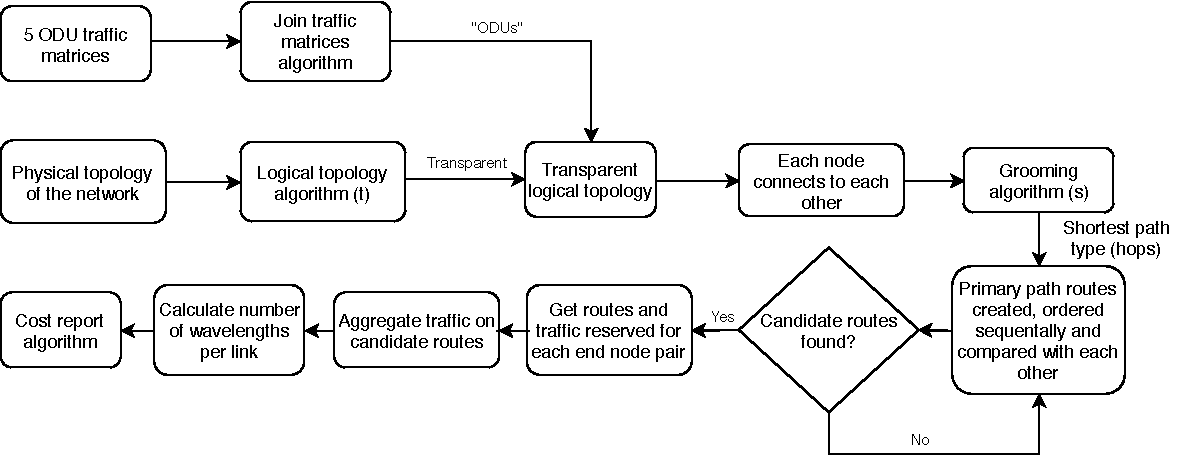
\includegraphics[width=16cm]{sdf/heuristic/transparent/figures/fluxogram_transparent_surv}
\caption{Fluxogram with the steps performed in the transparent without survivability transport mode approach.}
\label{fluxogram_transp_surv}
\end{figure}

\newpage
\subsubsection{Creation and join the traffic matrices}

\noindent
The first step is to create the traffic matrices based on the reference network \ref{Reference_Network_Topology}. In order to create the 5 traffic matrices in Net2Plan it is necessary the length of all the links and the total traffic used in this network, so later it is needed to define in Net2Plan the length in all end nodes and the total traffic depends on the value of traffic used (low traffic - 0.5 Tbit/s, medium traffic - 5 Tbit/s and high traffic - 10 Tbit/s). As you can see in the figure below, it is defined the path of the 5 ODUs and they will be aggregated in just one single ODU, making it possible to join all the demands in just one file and load it later into the network. This final resulting ODU joins the multiple traffic demands from all the traffic matrices previously created and, of course, the traffic demands will depend on the values used on the creation of the matrices (low, medium and high traffic).

\begin{figure}[H]
\centering
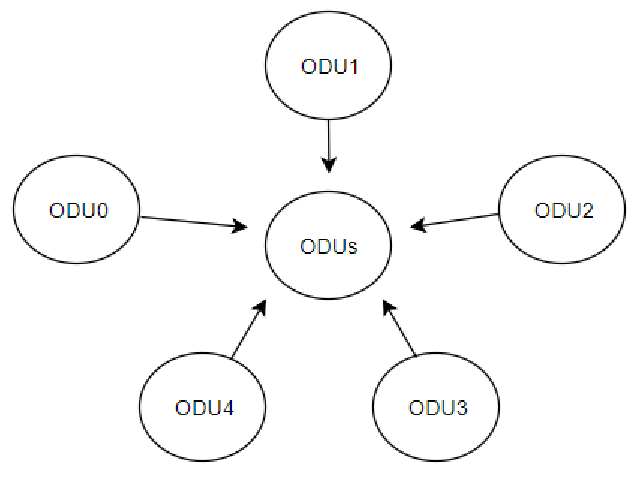
\includegraphics[width=7cm]{sdf/heuristic/transparent/figures/join_matrices_odus}
\caption{Join the 5 ODU traffic matrices into 1 single file "ODUs". The 5 traffic demands from the traffic matrices previously created are joined into 1 file to load it later on Net2Plan.}
\label{join_matrices_odus_transp_protec}
\end{figure}

\begin{figure}[H]
\centering
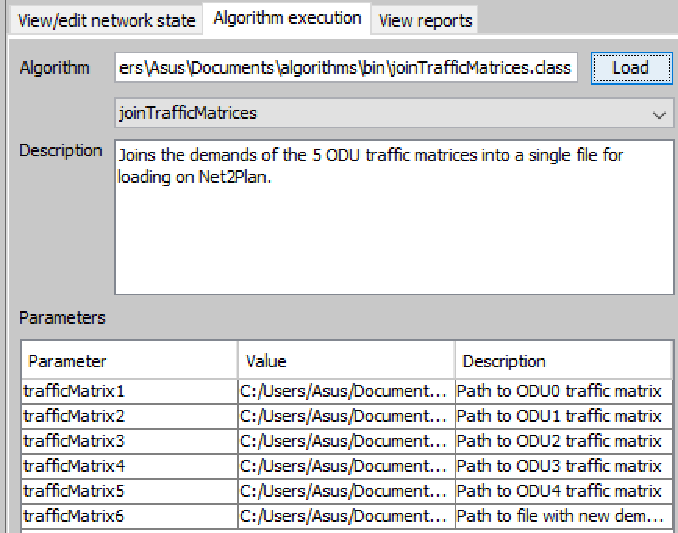
\includegraphics[width=8cm]{sdf/heuristic/transparent/figures/traffic_matrices}
\caption{Load of the join traffic matrices algorithm for the transparent transport mode on Net2Plan. It is defined the 5 paths to load the 5 ODU traffic matrices and the last path is the one where will be saved the file that joins all 5 the traffic demands.}
\label{traffic_matrices_transp_surv_ref}
\end{figure}

\newpage
\subsubsection{Creation of the physical topology}

\vspace{11pt}
The next step is to create the allowed physical topology of the network in Net2Plan. This network consists in 6 nodes and 8 bidirectional links. It is now also possible to define the length in all links. In the figure below it is shown the allowed physical topology in this transport mode.

\begin{figure}[H]
\centering
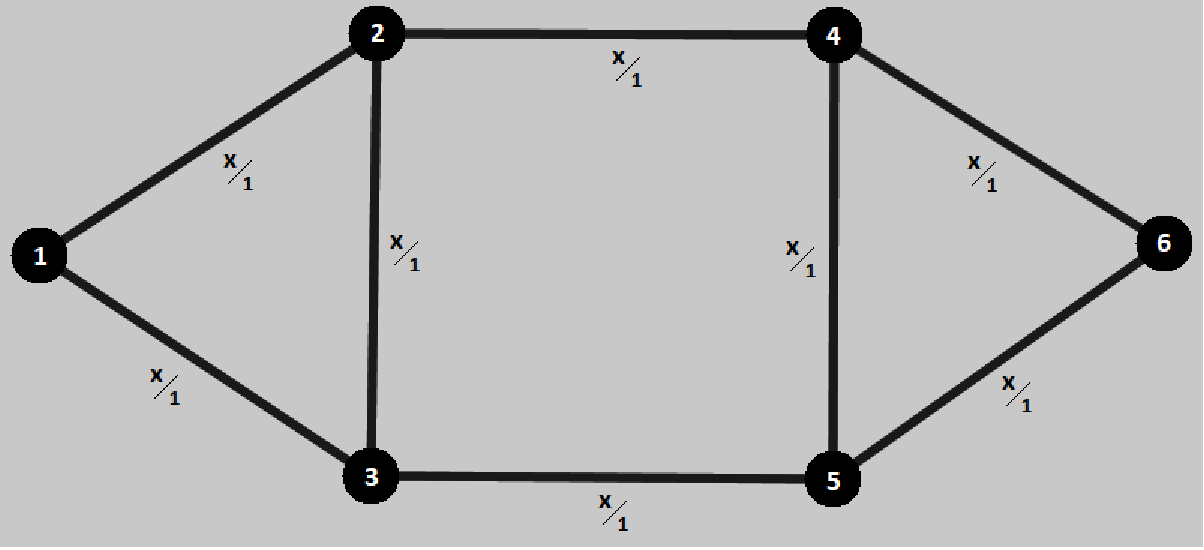
\includegraphics[width=12cm]{sdf/heuristic/transparent/figures/allowed_physical}
\caption{Allowed physical topology. The allowed physical topology is defined by the duct and sites in the field. It is assumed that each duct supports up to 1 bidirectional transmission system and each site supports up to 1 node.}
\label{allowed_physical_surv_transp}
\end{figure}

\subsubsection{Creation of the logical topology}

\vspace{11pt}
It is now time to create the allowed logical topology. A network topology represents how the links and the nodes of the network interconnect with each other and the logical topology algorithm creates the logical topology on another layer. In the transparent transport mode each node connects to each other creating direct links between all nodes in the network. Going through all nodes, if a node has a different index from other one, then creates a shortest and direct link between them. These additions of links between end nodes are made in the new upper layer of the network. The respective demands are saved in the new upper layer and those demands from the lower layer are then removed. The lower layer is the physical layer of the network and it is now created a new upper layer which is the logical layer of the network and represents the logical topology of the transparent transport mode.
The allowed physical and optical topologies, the logical topologies for all ODUs and the resulting physical topology is shown in the next section below \ref{result_description_transparent_heuristic_surv} for the three traffic scenarios. It is shown below three figures with the code in Java of the creation of the network logical topology, the load of the logical topology algorithm in Net2Plan and the resulting allowed optical topology for the transparent transport mode without survivability.

\begin{figure}[H]
\centering
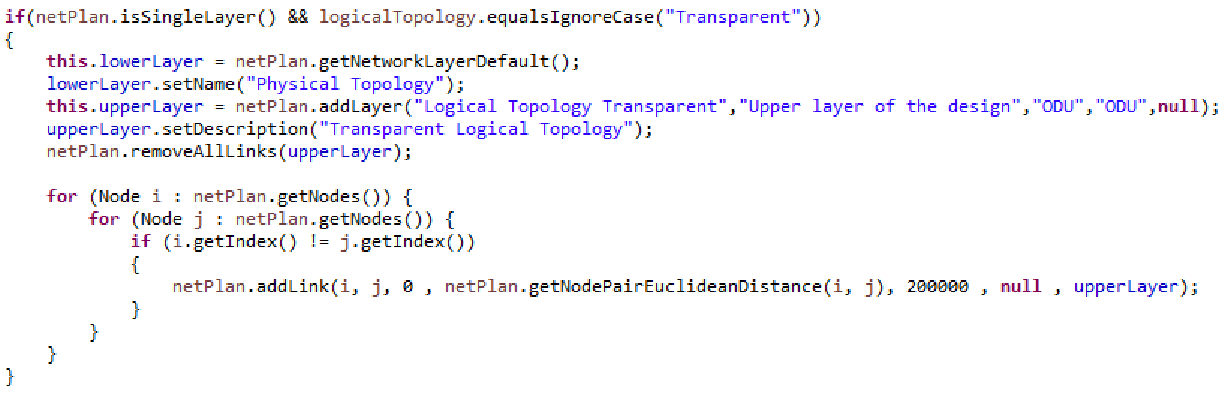
\includegraphics[width=15cm]{sdf/heuristic/transparent/figures/logical_topology_creation_transparent}
\caption{Java code of the logical topology approach for the transparent transport mode. The logical layer is created by adding direct links between all end nodes. The new layer is now the transparent logical topology of the network.}
\label{logical_topology_creation_transparent_surv}
\end{figure}

\begin{figure}[H]
\centering
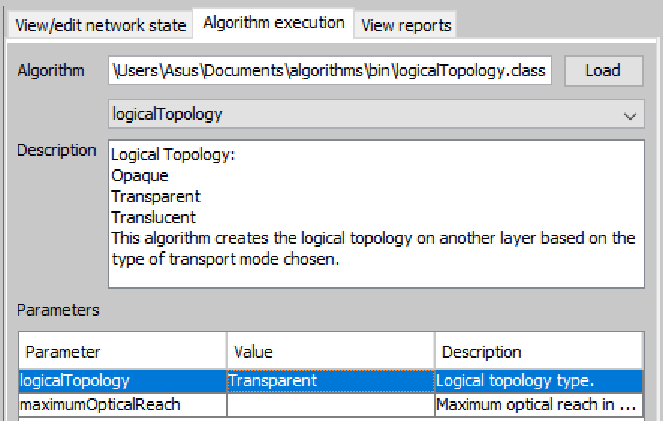
\includegraphics[width=10cm]{sdf/heuristic/transparent/figures/logical_topology_load_transparent}
\caption{Load of the logical topology algorithm for the transparent transport mode.}
\label{logical_topology_load_transparent_surv}
\end{figure}

\begin{figure}[H]
\centering
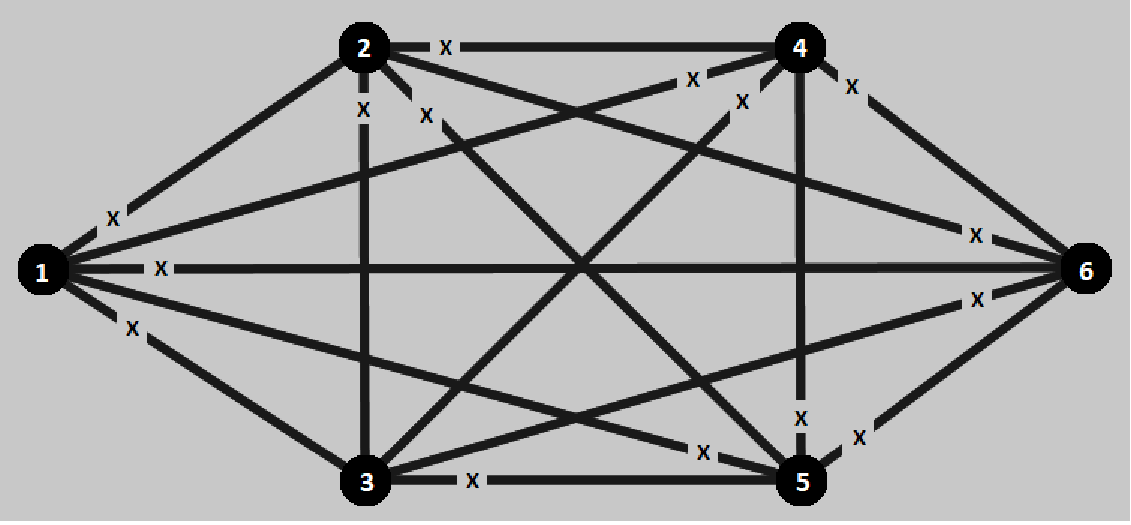
\includegraphics[width=10cm]{sdf/heuristic/transparent/figures/allowed_optical}
\caption{Allowed optical topology. It is assumed that each connections between demands supports up to 100 lightpaths.}
\label{allowed_optical_surv_transparent}
\end{figure}

\subsubsection{Creation of routes and aggregation of traffic}

\vspace{11pt}
After a network topology is created, it is now time to set the routing algorithm. In the transparent without survivability transport mode the routing algorithm is similar with the one used in opaque transport mode. It starts with going through all the demands and nodes which have different index between them (end nodes), create bidirectional routes (in this case the primary paths) based on the shortest path Dijkstra algorithm and then search the candidate routes for the respective demand. In this report it is used the shortest path type in hops. These routes are ordered sequentially and the shortest one per each demand is the primary path. The demands from the lower layer are removed and then saved in the upper layer. After this step, the routes are saved to a "Set" \ of routes and in each link of end nodes it is set the traffic demands into these routes that will integrate the whole network.

\begin{figure}[H]
\centering
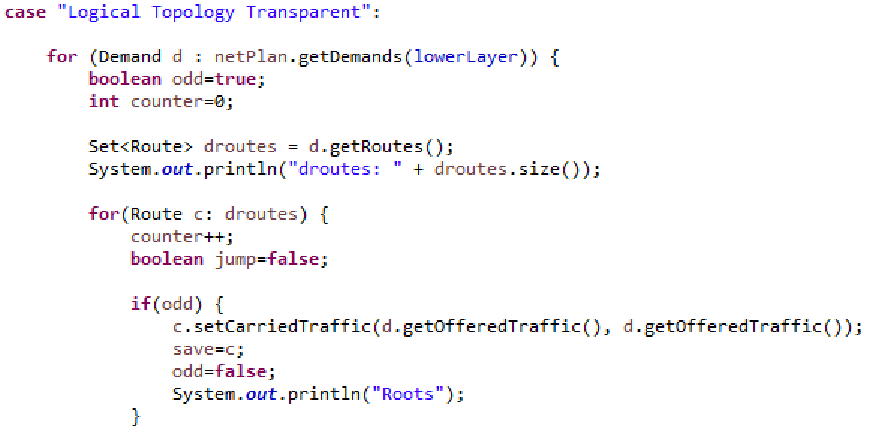
\includegraphics[width=14cm]{sdf/heuristic/transparent/figures/grooming_transparent_surv1}
\caption{Creation of routes and aggregation of traffic for the transparent without survivability transport mode. The candidate routes are searched by the shortest path type method and the offered traffic demands are set into these routes.}
\label{grooming_transparent_surv1}
\end{figure}

\begin{figure}[H]
\centering
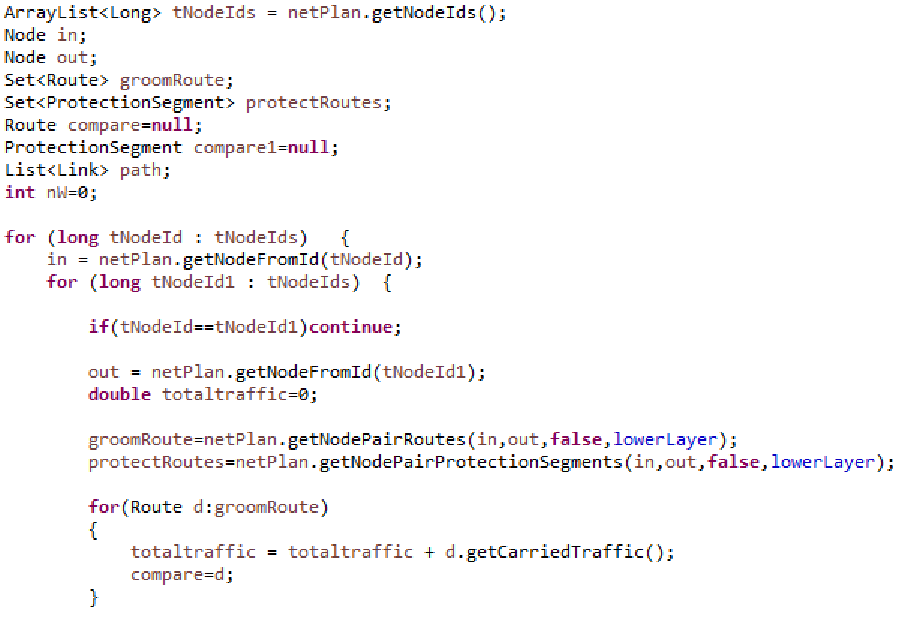
\includegraphics[width=14cm]{sdf/heuristic/transparent/figures/grooming_transparent_surv2}
\caption{Creation of routes and aggregation of traffic for the transparent without survivability transport mode. The traffic demands are set into the candidate primary path routes found earlier.}
\label{grooming_transparent_surv2}
\end{figure}

\begin{table}[H]
\centering
\begin{tabular}{|| c | c ||}
 \hline
 Function & Definition \\
 \hline\hline
 netPlan.getDemands(lowerLayer) & Returns the array of demands for the lower layer. \\
 \hline
 d.getRoutes() & Returns all the routes associated to the demand "d". \\
 \hline
 c.setCarriedTraffic() & \makecell{Sets the route carried traffic and the occupied capacity\\in the links, setting it up to be the same in all links.} \\
 \hline
 d.getOfferedTraffic() & Returns the offered traffic of the demand "d". \\
 \hline
 netPlan.getNodeIds() & Returns the array of the nodes' indexes. \\
 \hline
 netPlan.getNodeFromId(tNodeId) & Returns the node with the index "tNodeId". \\
 \hline
 \makecell{netPlan.getNodePairRoutes\\(in,out,false,lowerLayer)} &  \makecell{Returns the routes at "lowerLayer" \ \\from nodes "in" \ and "out".} \\
 \hline
\end{tabular}
\caption{Table with the description of the main functions in the creation of routes and aggregation of traffic in the grooming algorithm.}
\label{grooming_table_variables_transparent_surv}
\end{table}

\newpage
\subsubsection{Calculation of the number of wavelengths per link}

\vspace{11pt}
The final step of the routing and grooming algorithms is to calculate the number of wavelengths per link for the whole network. This is the last and an important step because with the number of wavelengths per link in the network, it is possible to calculate other network components. In the transparent transport mode, as in the figure below shows, the algorithm starts with going through all the nodes which have different index between them (end nodes) and in all the links that crosses between these pairs of nodes is reserved a link capacity based on the previous traffic aggregation. The total carried traffic in the link including protection and non-protection segments will be divided by the wavelength capacity and it is now possible to obtain the number of wavelengths per link.

\begin{figure}[H]
\centering
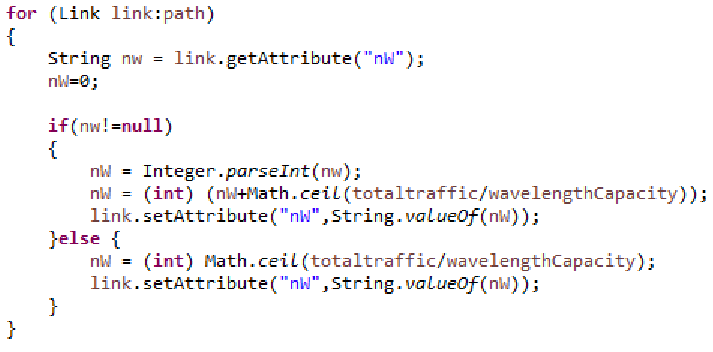
\includegraphics[width=13cm]{sdf/heuristic/transparent/figures/grooming_transparent_surv3}
\caption{Calculation of the number of wavelengths per link for the transparent transport mode. The link capacity is reserved based on the previous traffic aggregation.}
\label{grooming_transparent_surv3}
\end{figure}

\begin{figure}[H]
\centering
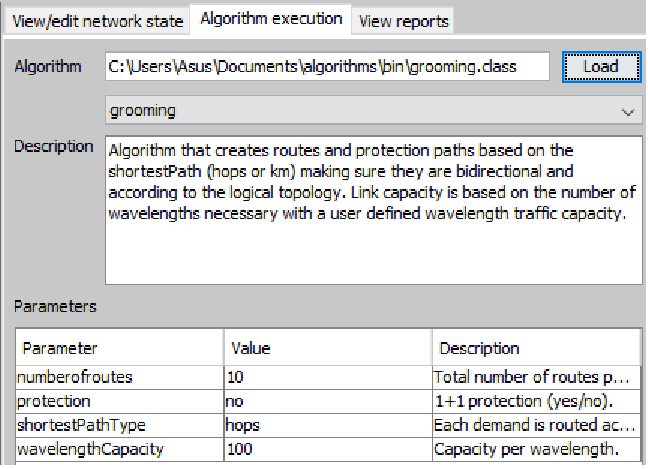
\includegraphics[width=11cm]{sdf/heuristic/transparent/figures/grooming_transparent_surv4}
\caption{Load of the grooming algorithm for the transparent without survivability transport mode. The total number of routes per demand is set to 10, the user can define if the model is with or without protection, the shortest path type is set to "hops" \ and the capacity per wavelength is used 100 optical channels.}
\label{grooming_transparent_surv4}
\end{figure}

\newpage
\subsubsection{Network cost report}

\vspace{11pt}
In order to obtain the network CAPEX results, the formulas needed to calculate the network elements and that are demonstrated previously in the beginning of this section \ref{heuristic_Transp_Survivability} were "translated" \ into Java code in a cost report algorithm. This algorithm can be loaded in Net2Plan and calculates and shows in tables the network CAPEX and also the per-link and per-node information with more details.

\begin{figure}[H]
\centering
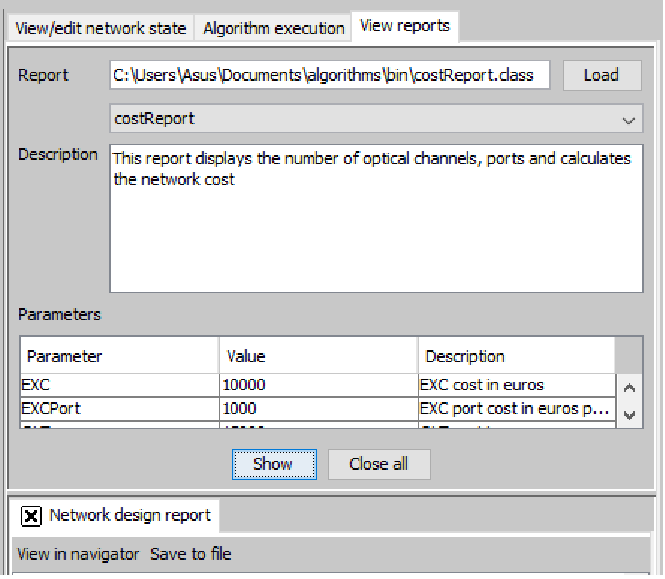
\includegraphics[width=10cm]{sdf/heuristic/transparent/figures/cost_report_transparent}
\caption{Load of the cost report algorithm on Net2Plan. The result view is an HTML page with the network optical and electrical components and their costs.}
\label{cost_report_transparent_surv}
\end{figure}

\newpage
\subsubsection{Result description}\label{result_description_transparent_heuristic_surv}

It is already known all the necessary formulas to obtain the CAPEX value for the reference network \ref{Reference_Network_Topology}. As described in the subsection of the network traffic \ref{Reference_Network_Traffic}, it is necessary to obtain three different values of CAPEX for the low (0.5 Tbit/s), medium (5 Tbit/s) and high (10 Tbit/s) traffic. It is used a network software program called Net2Plan which can design the traffic matrices, create all the network topologies, simulate the algorithms into the network implemented in the programming software called Eclipse and analyze the results obtained.\\
In this chapter will be demonstrated the results by Vasco's heuristics from 2016. In each of the three traffic scenarios, it will be shown the network topologies followed by the table with the CAPEX value of the network.\\

\noindent
\textbf{Low Traffic Scenario:}\\

In this scenario we have to take into account the traffic calculated in \ref{low_scenario}. In a first phase we will show the various existing topologies of the network. The first are the allowed topologies, physical and optical topologies, the second are the logical topology for all ODUs and finally the resulting physical topology.\\

\begin{figure}[H]
\centering
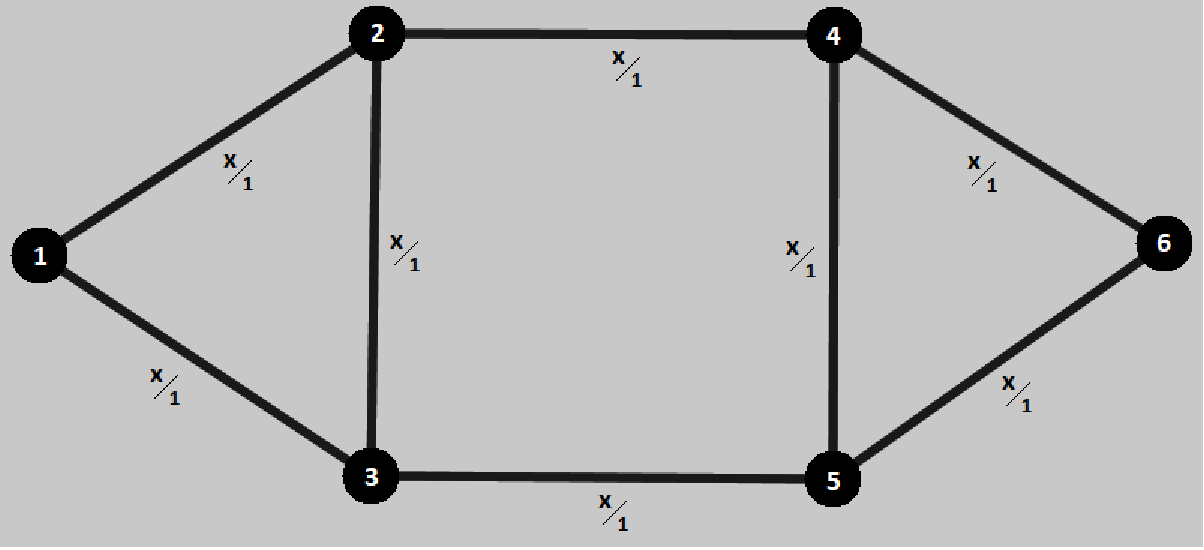
\includegraphics[width=13cm]{sdf/heuristic/transparent/figures/allowed_physical}
\caption{Allowed physical topology. The allowed physical topology is defined by the duct and sites in the field. It is assumed that each duct supports up to 1 bidirectional transmission system and each site supports up to 1 node.}
\label{allowed_physical_surv_ref_low_heuristic_transparent}
\end{figure}

\begin{figure}[H]
\centering
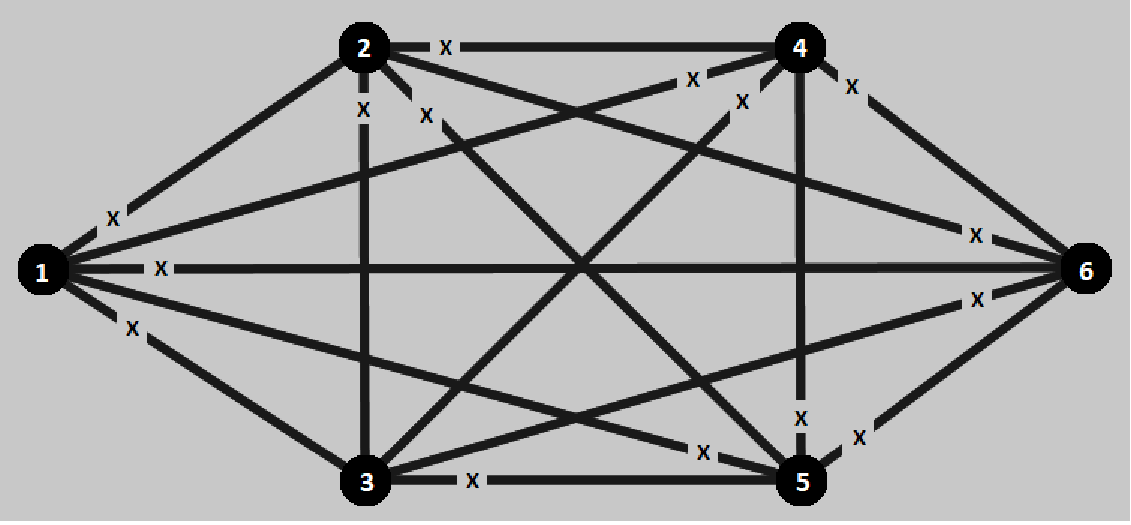
\includegraphics[width=13cm]{sdf/heuristic/transparent/figures/allowed_optical}
\caption{Allowed optical topology. The allowed optical topology is defined by the transport mode (transparent transport mode in this case). It is assumed that each connections between demands supports up to 100 lightpaths.}
\label{allowed_optical_surv_ref_low_heuristic_transparent}
\end{figure}

\begin{figure}[H]
\centering
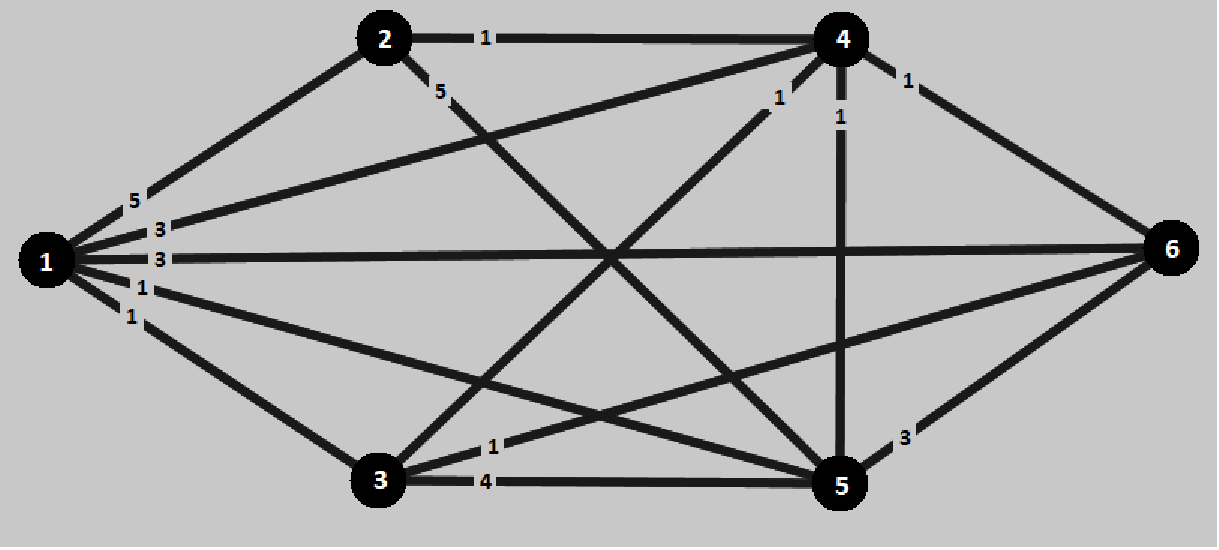
\includegraphics[width=13cm]{sdf/heuristic/transparent/figures/logical_topology_odu0_low}
\caption{ODU0 logical topology defined by the ODU0 traffic matrix.}
\label{logical_ODU0_surv_ref_low_heuristic_transparent}
\end{figure}

\begin{figure}[H]
\centering
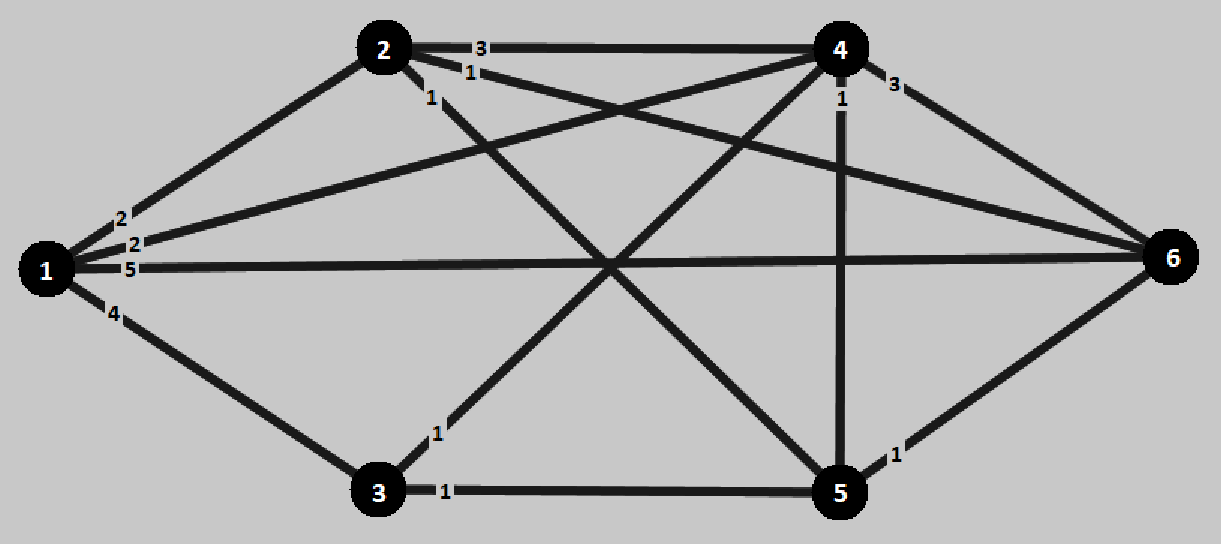
\includegraphics[width=13cm]{sdf/heuristic/transparent/figures/logical_topology_odu1_low}
\caption{ODU1 logical topology defined by the ODU1 traffic matrix.}
\label{logical_ODU1_surv_ref_low_heuristic_transparent}
\end{figure}

\begin{figure}[H]
\centering
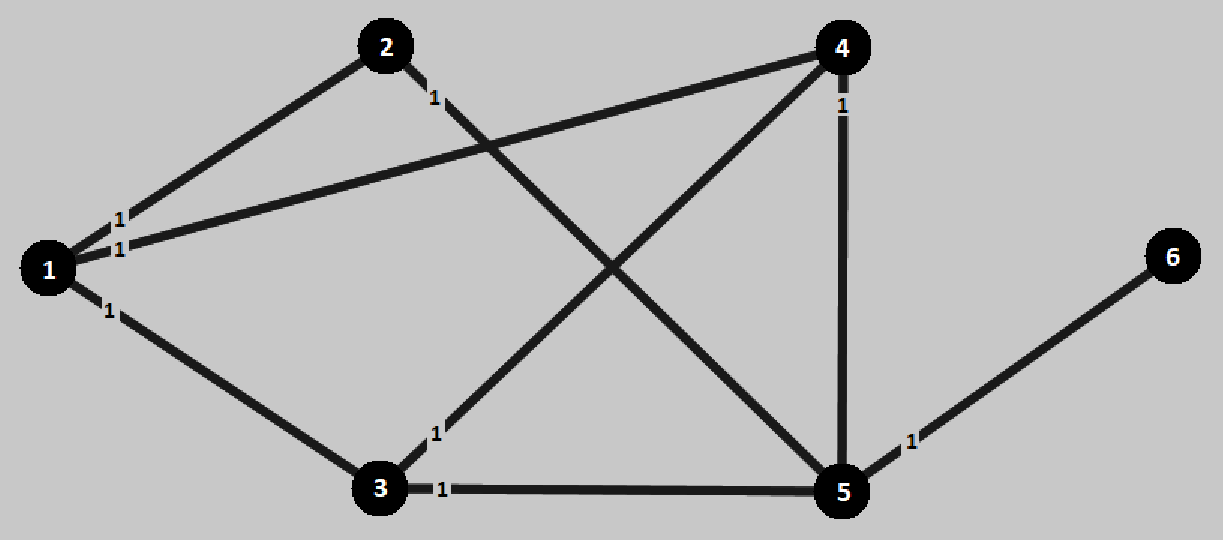
\includegraphics[width=13cm]{sdf/heuristic/transparent/figures/logical_topology_odu2_low}
\caption{ODU2 logical topology defined by the ODU2 traffic matrix.}
\label{logical_ODU2_surv_ref_low_heuristic_transparent}
\end{figure}

\begin{figure}[H]
\centering
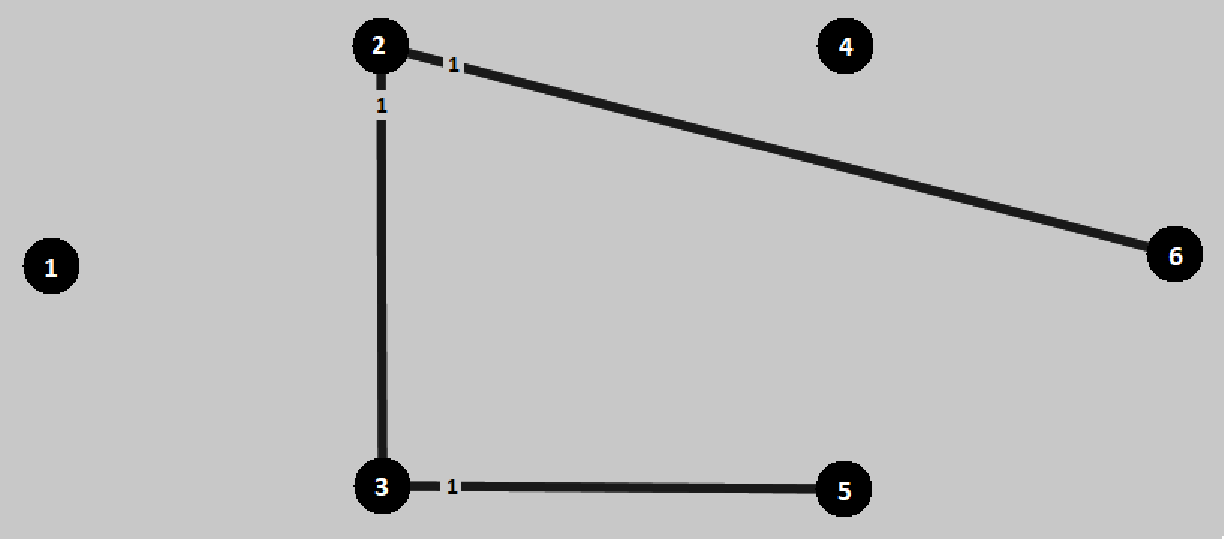
\includegraphics[width=13cm]{sdf/heuristic/transparent/figures/logical_topology_odu3_low}
\caption{ODU3 logical topology defined by the ODU3 traffic matrix.}
\label{logical_ODU3_surv_ref_low_heuristic_transparent}
\end{figure}

\begin{figure}[H]
\centering
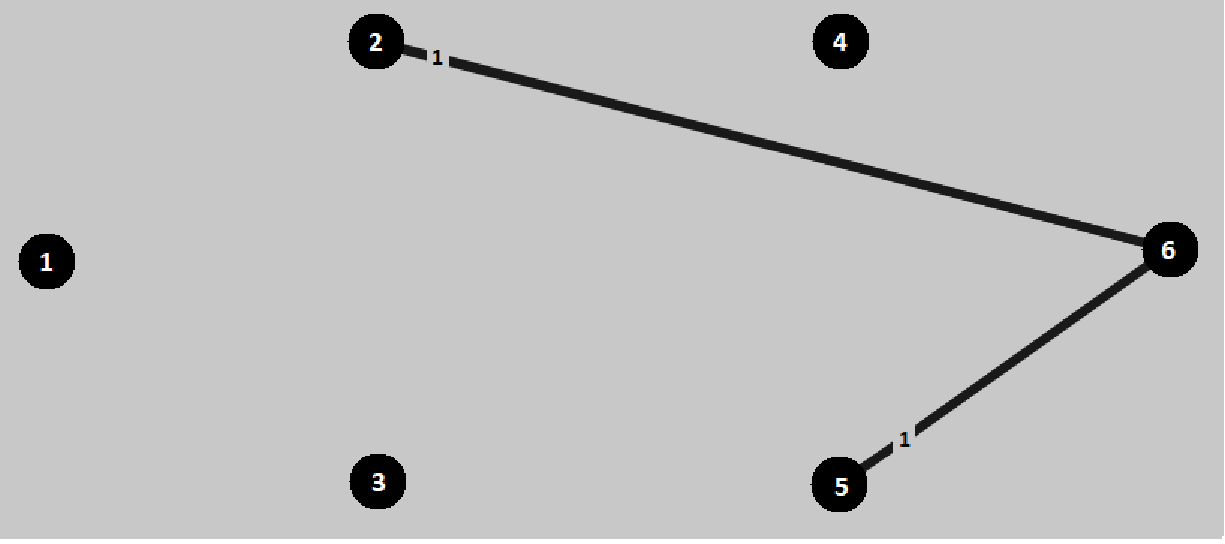
\includegraphics[width=13cm]{sdf/heuristic/transparent/figures/logical_topology_odu4_low}
\caption{ODU4 logical topology defined by the ODU4 traffic matrix.}
\label{logical_ODU4_surv_ref_low_heuristic_transparent}
\end{figure}

\begin{figure}[H]
\centering
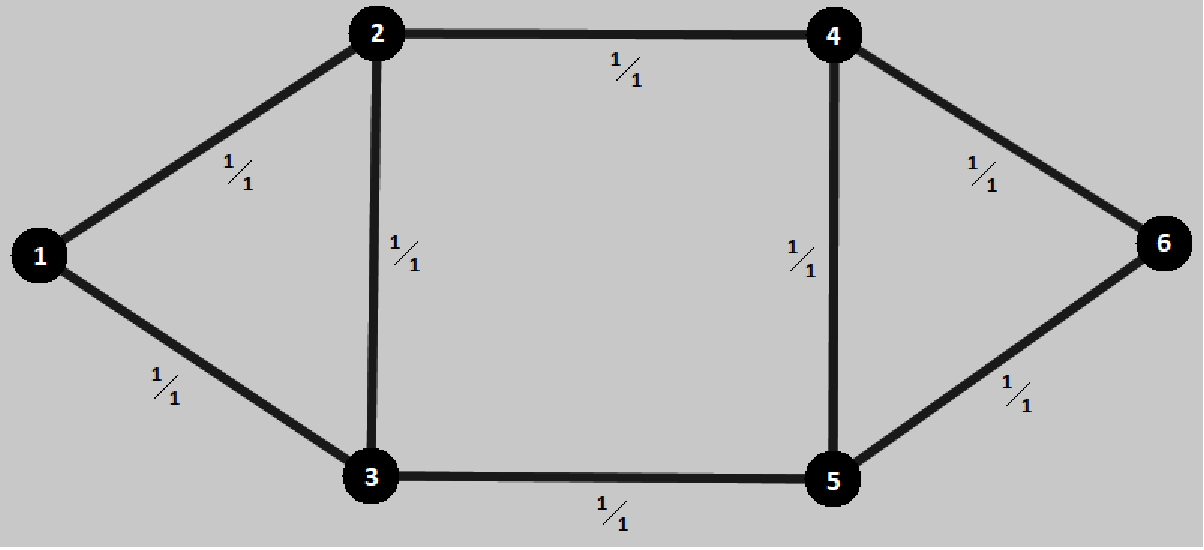
\includegraphics[width=13cm]{sdf/heuristic/transparent/figures/physical_topology}
\caption{Physical topology after dimensioning.}
\label{physical_topology_surv_ref_low_heuristic_transparent}
\end{figure}

Following all the steps mentioned in the \ref{net2plan_guide}, applying the routing and grooming heuristic algorithms in the Net2Plan software and using all the data referring to this scenario, the obtained result for the Vasco's heuristics can be consulted in the following table \ref{scripttransp_surv_ref_low_heuristic}.\\

\begin{table}[H]
\centering
\begin{tabular}{|| c | c | c | c | c | c | c ||}
 \hline
 \multicolumn{7}{|| c ||}{CAPEX of the Network} \\
 \hline
 \hline
 \multicolumn{3}{|| c |}{ } & Quantity & Unit Price & Cost & Total \\
 \hline
 \multirow{3}{*}{\makecell{Link \\ Cost}} & \multicolumn{2}{ c |}{OLTs} & 16 & 15 000 \euro & 240 000 \euro & \multirow{3}{*}{26 520 000 \euro} \\ \cline{2-6}
 & \multicolumn{2}{ c |}{100 Gbits/s Transceivers} & 52 & 5 000 \euro/Gbit/s & 26 000 000 \euro & \\ \cline{2-6}
 & \multicolumn{2}{ c |}{Amplifiers} & 70 & 4 000 \euro & 280 000 \euro & \\
 \hline
 \multirow{10}{*}{\makecell{Node \\ Cost}} & \multirow{7}{*}{Electrical} & EXCs & 6 & 10 000 \euro & 60 000 \euro & \multirow{10}{*}{3 797 590 \euro} \\ \cline{3-6}
  & & ODU0 Ports & 60 & 10 \euro/port & 600 \euro & \\ \cline{3-6}
 & & ODU1 Ports & 50 & 15 \euro/port & 750 \euro & \\ \cline{3-6}
 & & ODU2 Ports & 16 & 30 \euro/port & 480 \euro & \\ \cline{3-6}
 & & ODU3 Ports & 6 & 60 \euro/port & 360 \euro & \\ \cline{3-6}
 & & ODU4 Ports & 4 & 100 \euro/port & 400 \euro & \\ \cline{3-6}
 & & Transponders & 34 & 100 000 \euro/port & 3 400 000 \euro & \\ \cline{2-6}
 & \multirow{3}{*}{Optical} & OXCs & 6 & 20 000 \euro & 120 000 \euro & \\ \cline{3-6}
 & & Line Ports & 52 & 2 500 \euro/port & 130 000 \euro & \\ \cline{3-6}
 & & Add Ports & 34 & 2 500 \euro/port & 85 000 \euro & \\
 \hline
 \multicolumn{6}{|| c |}{Total Network Cost} & 30 317 590 \euro \\
\hline
\end{tabular}
\caption{Table with detailed description of CAPEX of Vasco's 2016 results.}
\label{scripttransp_surv_ref_low_heuristic}
\end{table}

\vspace{17pt}
All the values calculated in the previous table were obtained through the equations \ref{Capex_Link_heuristic} and \ref{Capex_Node_heuristic} referred to in section \ref{Heuristic_CAPEX}, but for a more detailed analysis we created table \ref{formulas_transp_heuristic} where we can see how all the parameters are calculated individually. \\

\begin{table}[h!]
\centering
\begin{tabular}{|| c | c ||}
 \hline
  & Equation used to calculate the cost \\ \hline
 OLTs & \(\displaystyle 2 \sum_{i=1}^{N}\sum_{j=i+1}^{N} L_{ij} \gamma_0^{OLT} \) \\ \hline
 Transceivers & \(\displaystyle 2 \sum_{i=1}^{N}\sum_{j=i+1}^{N} L_{ij} f_{ij}^{od} \gamma_1^{OLT} \tau \) \\ \hline
 Amplifiers & \(\displaystyle 2 \sum_{i=1}^{N}\sum_{j=i+1}^{N} L_{ij} N^R_{ij} c^R \) \\ \hline
 EXCs & \(\displaystyle \sum_{n=1}^N N_{exc,n} \gamma_{e0} \) \\ \hline
 ODU0 Port & \(\displaystyle \sum_{n=1}^{N} \sum_{d=1}^{N} N_{exc,n} D_{nd,0} \gamma_{e1,0} \) \\ \hline
 ODU1 Port & \(\displaystyle \sum_{n=1}^{N} \sum_{d=1}^{N} N_{exc,n} D_{nd,1} \gamma_{e1,1} \) \\ \hline
 ODU2 Port & \(\displaystyle \sum_{n=1}^{N} \sum_{d=1}^{N} N_{exc,n} D_{nd,2} \gamma_{e1,2} \)\\ \hline
 ODU3 Port & \(\displaystyle \sum_{n=1}^{N} \sum_{d=1}^{N} N_{exc,n} D_{nd,3} \gamma_{e1,3} \) \\ \hline
 ODU4 Port & \(\displaystyle \sum_{n=1}^{N} \sum_{d=1}^{N} N_{exc,n} D_{nd,4} \gamma_{e1,4} \) \\ \hline
 LR Transponders & \(\displaystyle \sum_{n=1}^{N} \sum_{j=1}^{N} N_{exc,n} \lambda_{od} \gamma_{e1,-1} \) \\ \hline
 OXCs & \(\displaystyle \sum_{n=1}^N N_{oxc,n} \gamma_{o0} \) \\ \hline
 Add Port & \(\displaystyle \sum_{n=1}^{N} \sum_{j=1}^{N} N_{oxc,n} \lambda_{od} \gamma_{o1} \) \\ \hline
 Line Port & \(\displaystyle \sum_{n=1}^{N} \sum_{j=1}^{N} N_{oxc,n} f_{ij}^{od} \gamma_{o1} \) \\ \hline
 CAPEX & The final cost is calculated by summing all previous results. \\
 \hline
 \end{tabular}
\caption{Table with description of calculation}
\label{formulas_transp_heuristic}
\end{table}

\noindent
\textbf{Medium Traffic Scenario:}\\

In this scenario we have to take into account the traffic calculated in \ref{medium_traffic_scenario}. In a first phase we will show the various existing topologies of the network. The first are the allowed topologies, physical and optical topologies, the second are the logical topology for all ODUs and finally the resulting physical topology.\\

\begin{figure}[H]
\centering
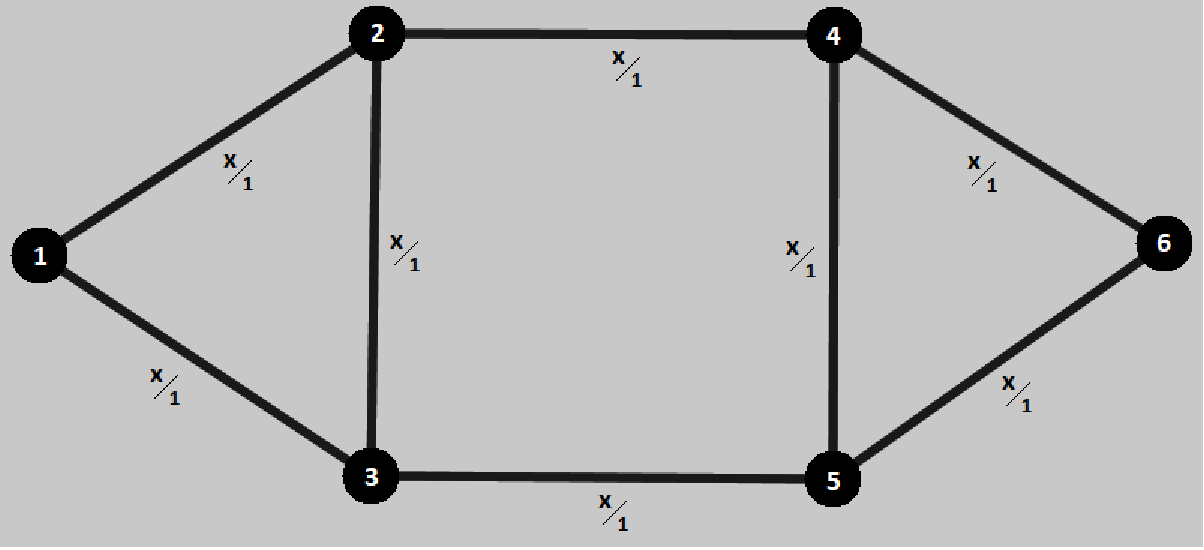
\includegraphics[width=13cm]{sdf/heuristic/transparent/figures/allowed_physical}
\caption{Allowed physical topology. The allowed physical topology is defined by the duct and sites in the field. It is assumed that each duct supports up to 1 bidirectional transmission system and each site supports up to 1 node.}
\label{allowed_physical_surv_ref_medium_heuristic_transparent}
\end{figure}

\begin{figure}[H]
\centering
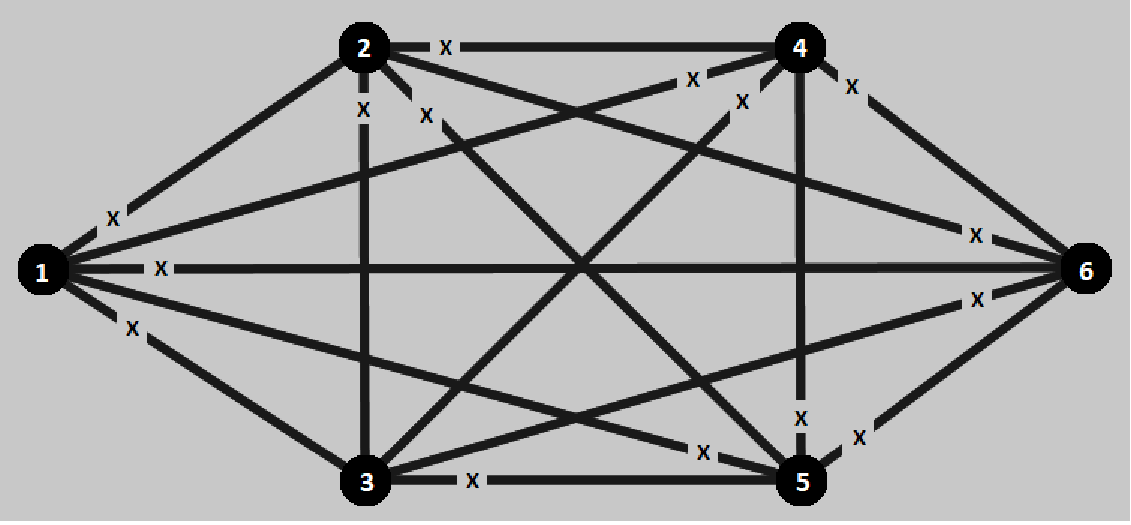
\includegraphics[width=13cm]{sdf/heuristic/transparent/figures/allowed_optical}
\caption{Allowed optical topology. The allowed optical topology is defined by the transport mode (transparent transport mode in this case). It is assumed that each connections between demands supports up to 100 lightpaths.}
\label{allowed_optical_surv_ref_medium_heuristic_transparent}
\end{figure}

\begin{figure}[H]
\centering
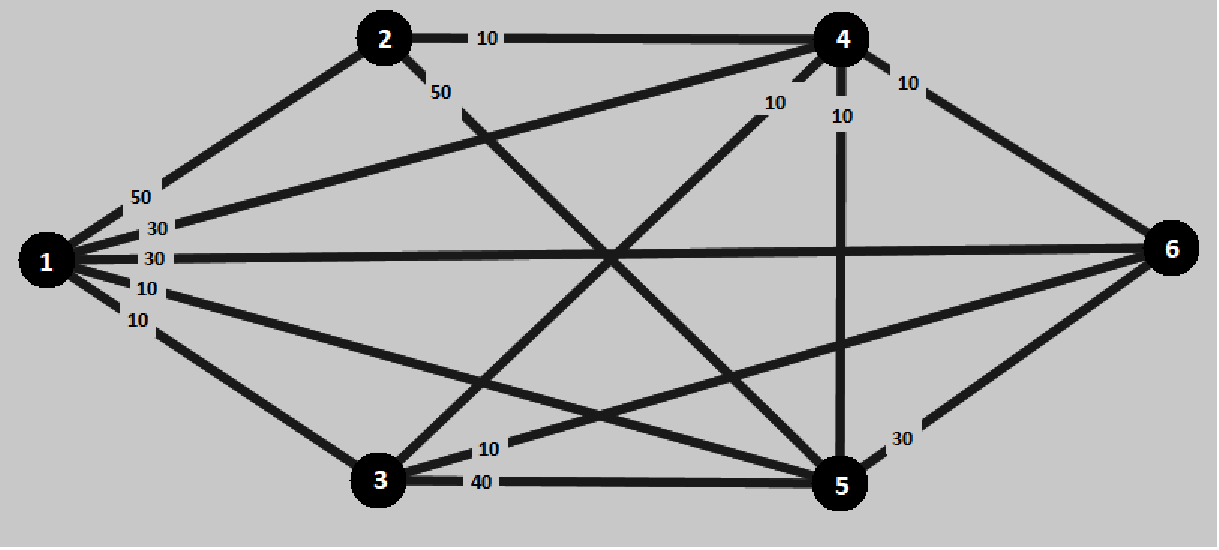
\includegraphics[width=13cm]{sdf/heuristic/transparent/figures/logical_topology_odu0_medium}
\caption{ODU0 logical topology defined by the ODU0 traffic matrix.}
\label{logical_ODU0_surv_ref_medium_heuristic_transparent}
\end{figure}

\begin{figure}[H]
\centering
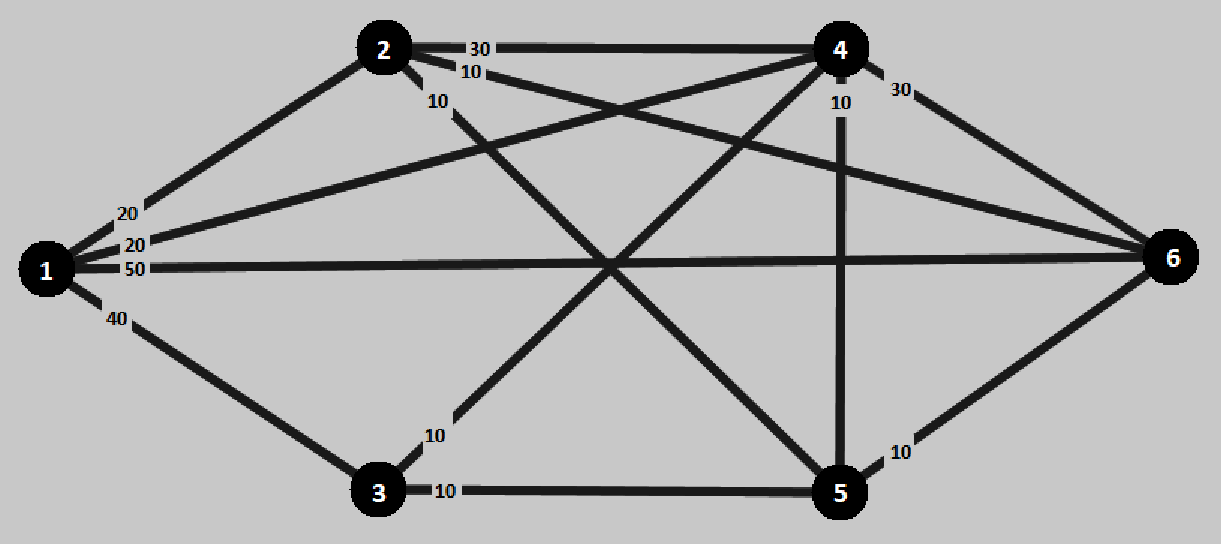
\includegraphics[width=13cm]{sdf/heuristic/transparent/figures/logical_topology_odu1_medium}
\caption{ODU1 logical topology defined by the ODU1 traffic matrix.}
\label{logical_ODU1_surv_ref_medium_heuristic_transparent}
\end{figure}

\begin{figure}[H]
\centering
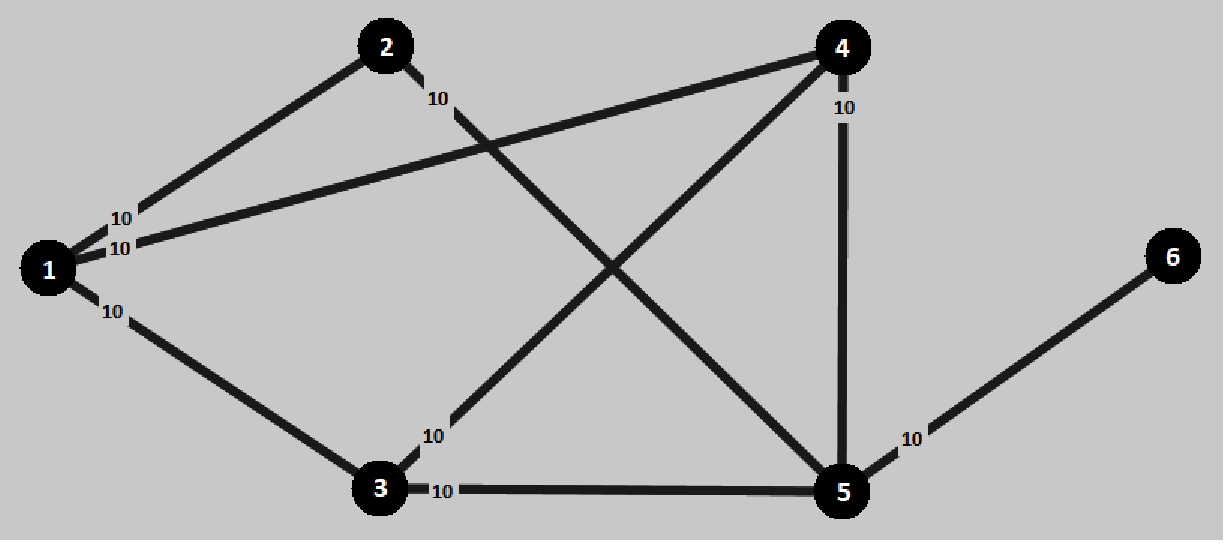
\includegraphics[width=13cm]{sdf/heuristic/transparent/figures/logical_topology_odu2_medium}
\caption{ODU2 logical topology defined by the ODU2 traffic matrix.}
\label{logical_ODU2_surv_ref_medium_heuristic_transparent}
\end{figure}

\begin{figure}[H]
\centering
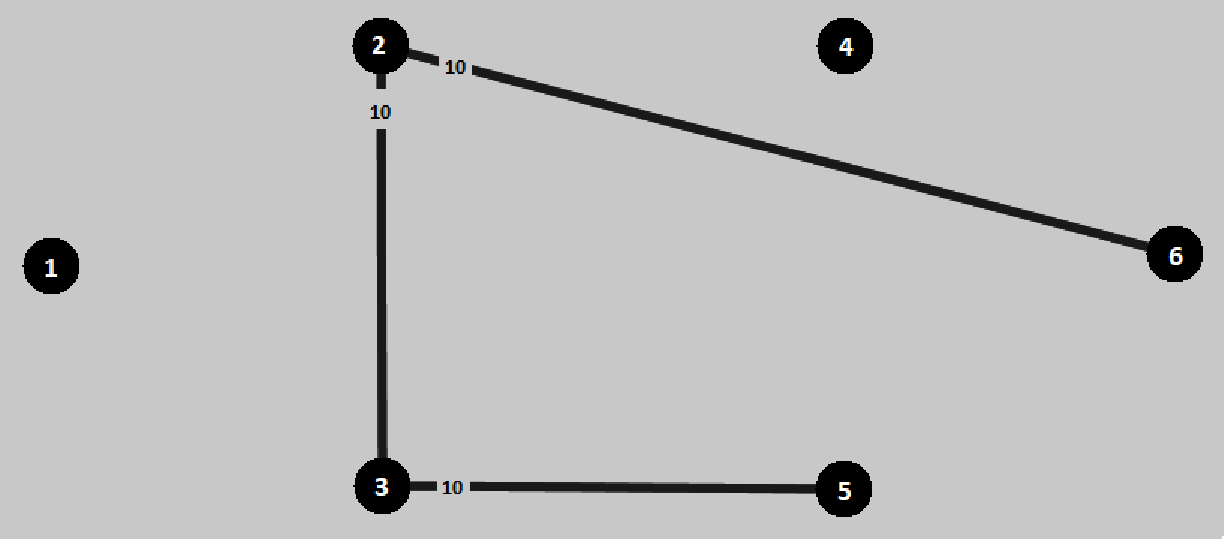
\includegraphics[width=13cm]{sdf/heuristic/transparent/figures/logical_topology_odu3_medium}
\caption{ODU3 logical topology defined by the ODU3 traffic matrix.}
\label{logical_ODU3_surv_ref_medium_heuristic_transparent}
\end{figure}

\begin{figure}[H]
\centering
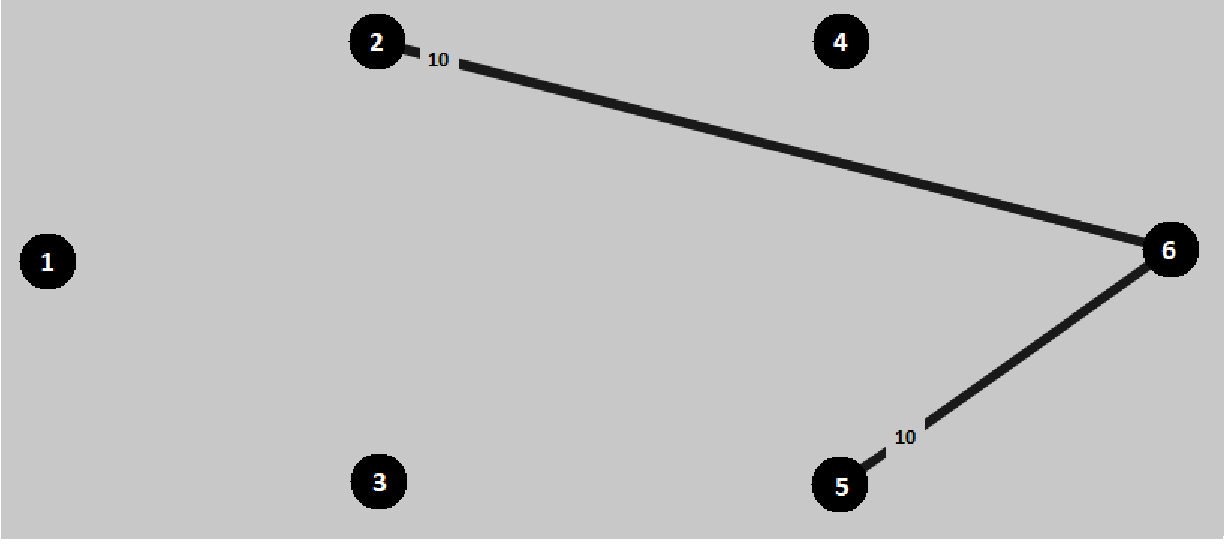
\includegraphics[width=13cm]{sdf/heuristic/transparent/figures/logical_topology_odu4_medium}
\caption{ODU4 logical topology defined by the ODU4 traffic matrix.}
\label{logical_ODU4_surv_ref_medium_heuristic_transparent}
\end{figure}

\begin{figure}[H]
\centering
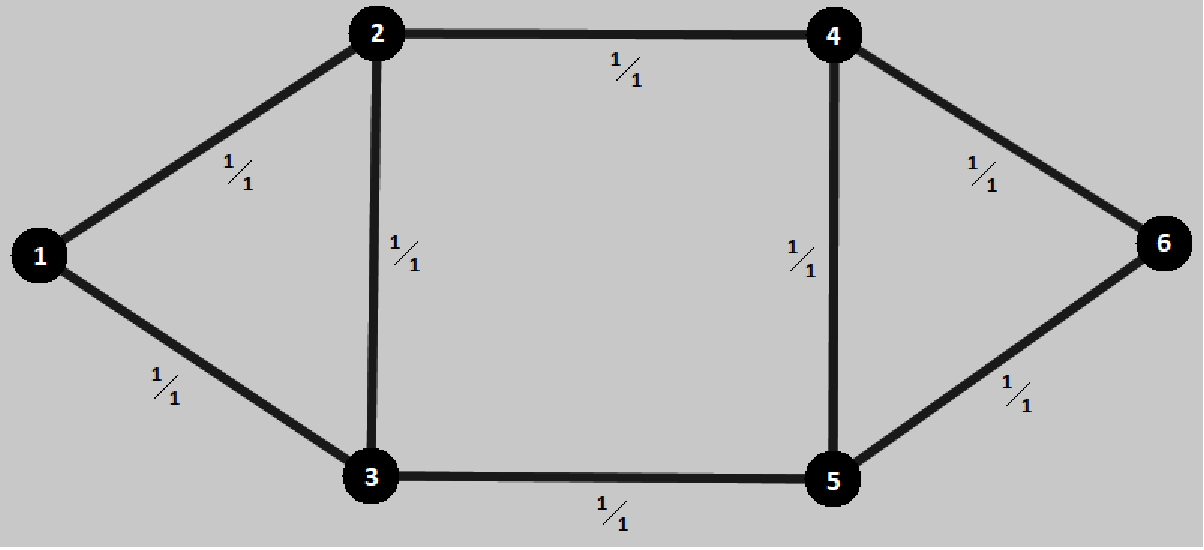
\includegraphics[width=13cm]{sdf/heuristic/transparent/figures/physical_topology}
\caption{Physical topology after dimensioning.}
\label{physical_topology_surv_ref_medium_heuristic_transparent}
\end{figure}

Following all the steps mentioned in the \ref{net2plan_guide}, applying the routing and grooming heuristic algorithms in the Net2Plan software and using all the data referring to this scenario, the obtained result for the Vasco's heuristics can be consulted in the following table \ref{scripttransp_surv_ref_medium_heuristic}. In table \ref{formulas_transp_heuristic} mentioned in previous scenario we can see how all the values were calculated. \\

\begin{table}[H]
\centering
\begin{tabular}{|| c | c | c | c | c | c | c ||}
 \hline
 \multicolumn{7}{|| c ||}{CAPEX of the Network} \\
 \hline
 \hline
 \multicolumn{3}{|| c |}{ } & Quantity & Unit Price & Cost & Total \\
 \hline
 \multirow{3}{*}{\makecell{Link \\ Cost}} & \multicolumn{2}{ c |}{OLTs} & 16 & 15 000 \euro & 240 000 \euro & \multirow{3}{*}{84 520 000 \euro} \\ \cline{2-6}
 & \multicolumn{2}{ c |}{100 Gbits/s Transceivers} & 168 & 5 000 \euro/Gbit/s & 84 000 000 \euro & \\ \cline{2-6}
 & \multicolumn{2}{ c |}{Amplifiers} & 70 & 4 000 \euro & 280 000 \euro & \\
 \hline
 \multirow{10}{*}{\makecell{Node \\ Cost}} & \multirow{7}{*}{Electrical} & EXCs & 6 & 10 000 \euro & 60 000 \euro & \multirow{10}{*}{15 180 900 \euro} \\ \cline{3-6}
 & & ODU0 Ports & 600 & 10 \euro/port & 6 000 \euro & \\ \cline{3-6}
 & & ODU1 Ports & 500 & 15 \euro/port & 7 500 \euro & \\ \cline{3-6}
 & & ODU2 Ports & 160 & 30 \euro/port & 4 800 \euro & \\ \cline{3-6}
 & & ODU3 Ports & 60 & 60 \euro/port & 3 600 \euro & \\ \cline{3-6}
 & & ODU4 Ports & 40 & 100 \euro/port & 4 000 \euro & \\ \cline{3-6}
 & & Transponders & 142 & 100 000 \euro/port & 14 200 000 \euro & \\ \cline{2-6}
 & \multirow{3}{*}{Optical} & OXCs & 6 & 20 000 \euro & 120 000 \euro & \\ \cline{3-6}
 & & Line Ports & 168 & 2 500 \euro/port & 420 000 \euro & \\ \cline{3-6}
 & & Add Ports & 142 & 2 500 \euro/port & 355 000 \euro & \\
 \hline
 \multicolumn{6}{|| c |}{Total Network Cost} & 99 700 900 \euro \\
\hline
\end{tabular}
\caption{Table with detailed description of CAPEX of Vasco's 2016 results.}
\label{scripttransp_surv_ref_medium_heuristic}
\end{table}

\noindent
\textbf{High Traffic Scenario:}\\

In this scenario we have to take into account the traffic calculated in \ref{high_traffic_scenario}. In a first phase we will show the various existing topologies of the network. The first are the allowed topologies, physical and optical topologies, the second are the logical topology for all ODUs and finally the resulting physical topology.\\

\begin{figure}[H]
\centering
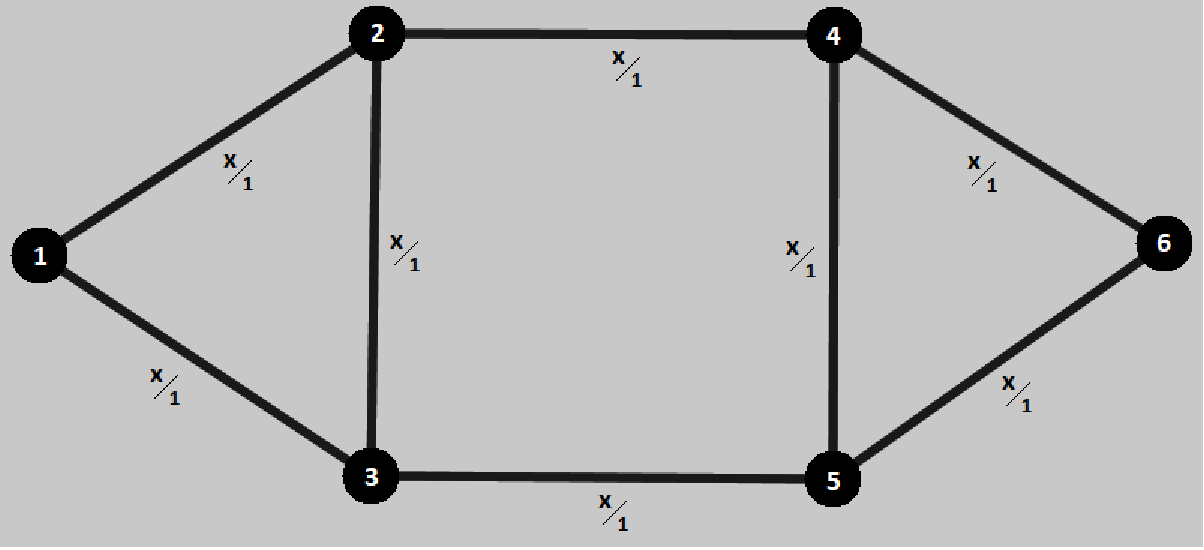
\includegraphics[width=13cm]{sdf/heuristic/transparent/figures/allowed_physical}
\caption{Allowed physical topology. The allowed physical topology is defined by the duct and sites in the field. It is assumed that each duct supports up to 1 bidirectional transmission system and each site supports up to 1 node.}
\label{allowed_physical_surv_ref_high_heuristic_transparent}
\end{figure}

\begin{figure}[H]
\centering
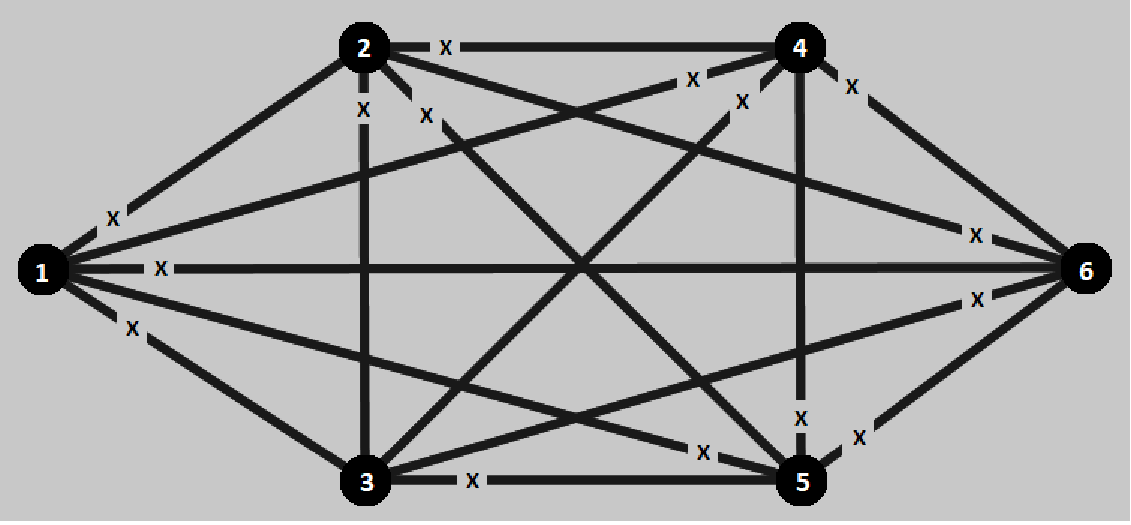
\includegraphics[width=13cm]{sdf/heuristic/transparent/figures/allowed_optical}
\caption{Allowed optical topology. The allowed optical topology is defined by the transport mode (transparent transport mode in this case). It is assumed that each connections between demands supports up to 100 lightpaths.}
\label{allowed_optical_surv_ref_high_heuristic_transparent}
\end{figure}

\begin{figure}[H]
\centering
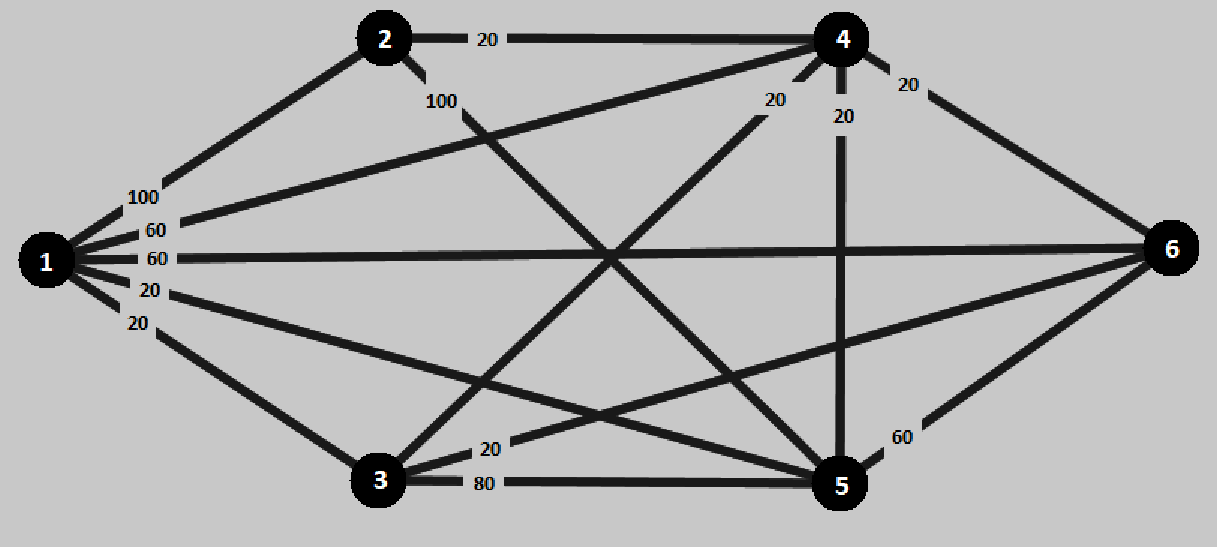
\includegraphics[width=13cm]{sdf/heuristic/transparent/figures/logical_topology_odu0_high}
\caption{ODU0 logical topology defined by the ODU0 traffic matrix.}
\label{logical_ODU0_surv_ref_high_heuristic_transparent}
\end{figure}

\begin{figure}[H]
\centering
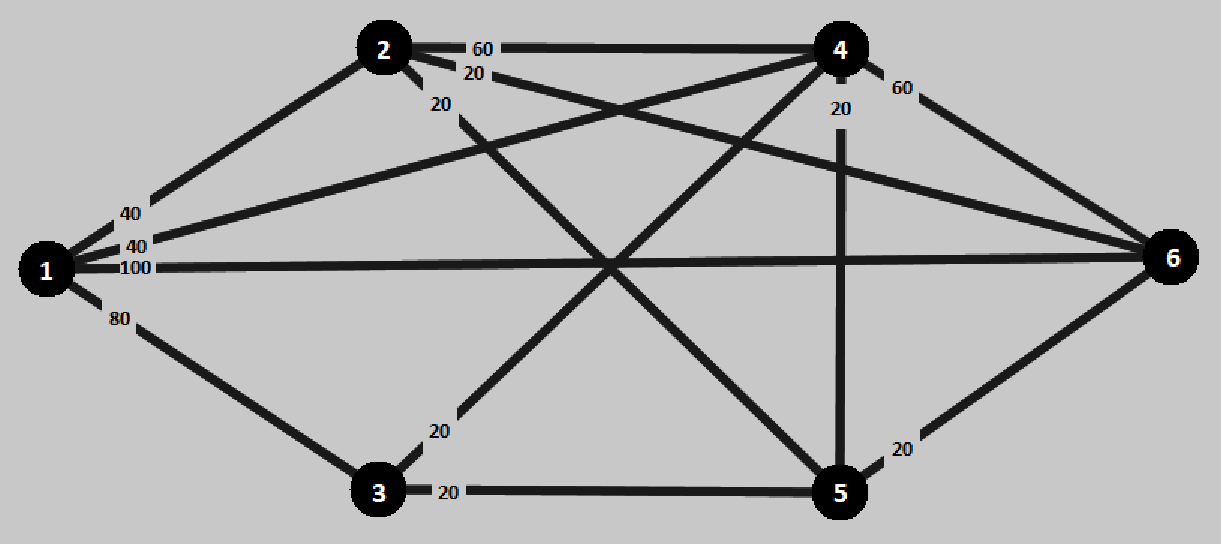
\includegraphics[width=13cm]{sdf/heuristic/transparent/figures/logical_topology_odu1_high}
\caption{ODU1 logical topology defined by the ODU1 traffic matrix.}
\label{logical_ODU1_surv_ref_high_heuristic_transparent}
\end{figure}

\begin{figure}[H]
\centering
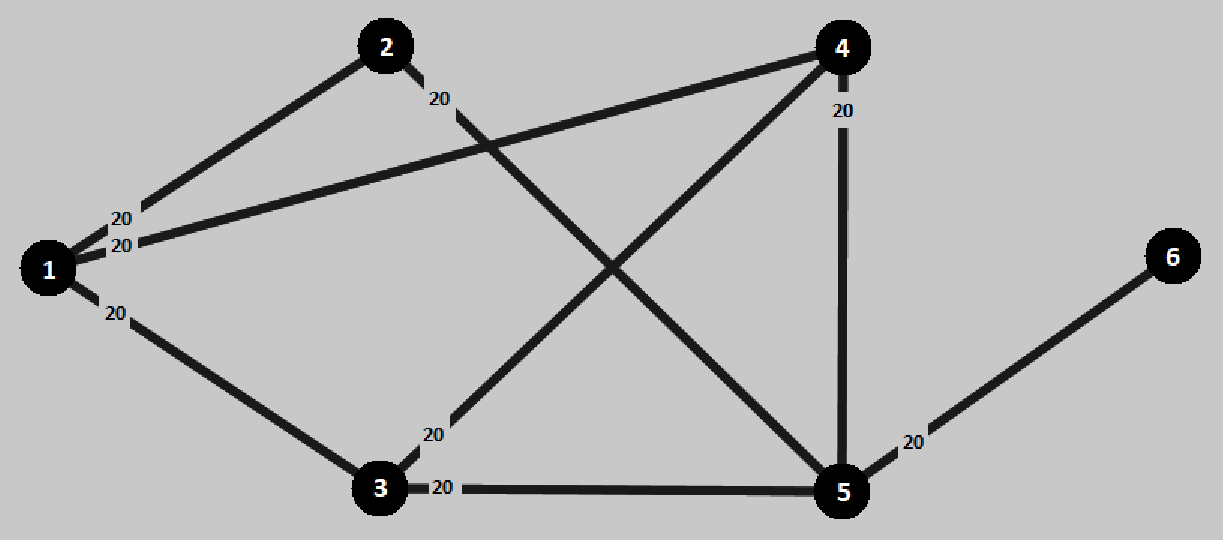
\includegraphics[width=13cm]{sdf/heuristic/transparent/figures/logical_topology_odu2_high}
\caption{ODU2 logical topology defined by the ODU2 traffic matrix.}
\label{logical_ODU2_surv_ref_high_heuristic_transparent}
\end{figure}

\begin{figure}[H]
\centering
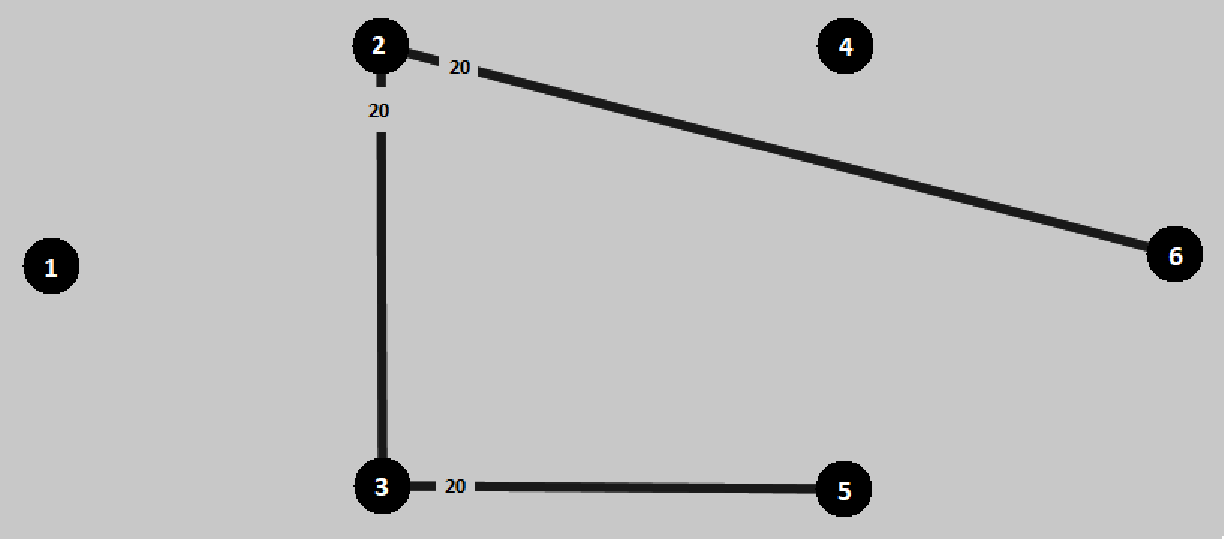
\includegraphics[width=13cm]{sdf/heuristic/transparent/figures/logical_topology_odu3_high}
\caption{ODU3 logical topology defined by the ODU3 traffic matrix.}
\label{logical_ODU3_surv_ref_high_heuristic_transparent}
\end{figure}

\begin{figure}[H]
\centering
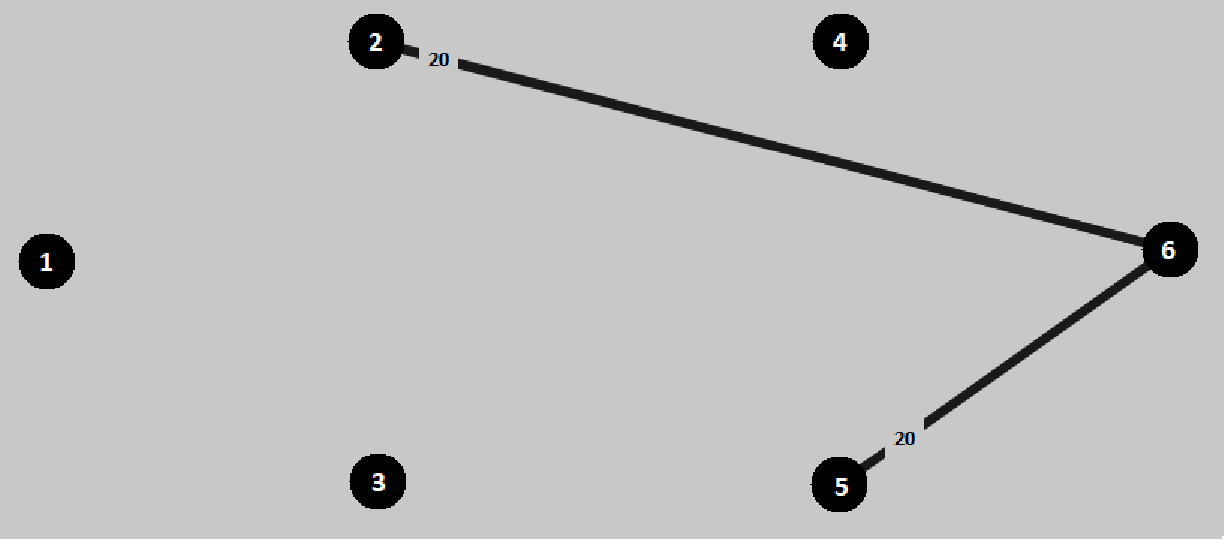
\includegraphics[width=13cm]{sdf/heuristic/transparent/figures/logical_topology_odu4_high}
\caption{ODU4 logical topology defined by the ODU4 traffic matrix.}
\label{logical_ODU4_surv_ref_high_heuristic_transparent}
\end{figure}

\begin{figure}[H]
\centering
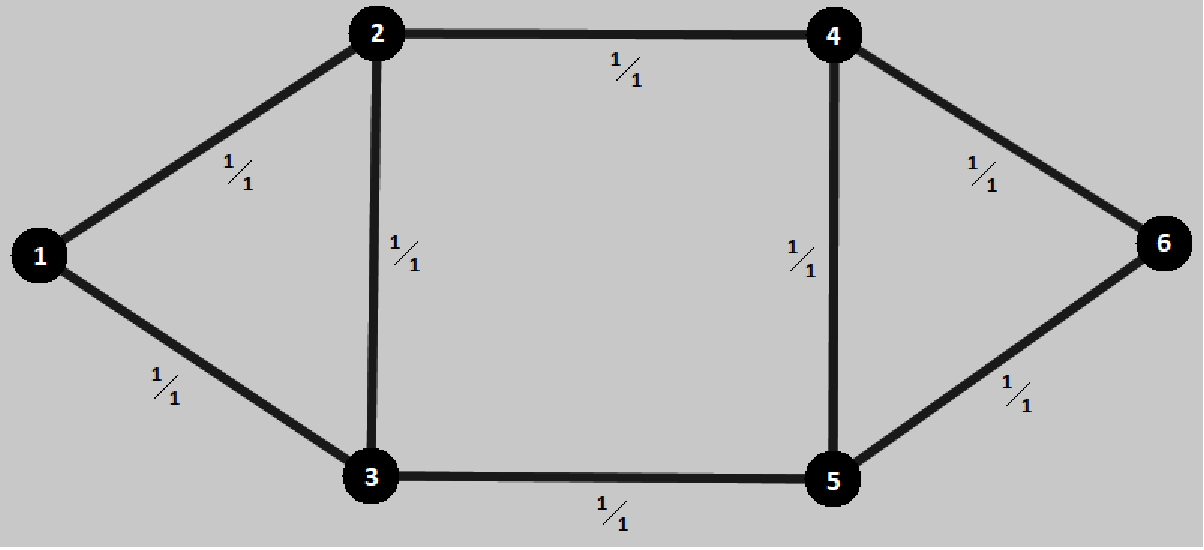
\includegraphics[width=13cm]{sdf/heuristic/transparent/figures/physical_topology}
\caption{Physical topology after dimensioning.}
\label{physical_topology_surv_ref_high_heuristic_transparent}
\end{figure}

Following all the steps mentioned in the \ref{net2plan_guide}, applying the routing and grooming heuristic algorithms in the Net2Plan software and using all the data referring to this scenario, the obtained result for the Vasco's heuristics can be consulted in the following table \ref{scripttransp_surv_ref_high_heuristic}. In table \ref{formulas_transp_heuristic} mentioned in previous scenario we can see how all the values were calculated. \\

\begin{table}[H]
\centering
\begin{tabular}{|| c | c | c | c | c | c | c ||}
 \hline
 \multicolumn{7}{|| c ||}{CAPEX of the Network} \\
 \hline
 \hline
 \multicolumn{3}{|| c |}{ } & Quantity & Unit Price & Cost & Total \\
 \hline
 \multirow{3}{*}{\makecell{Link \\ Cost}} & \multicolumn{2}{ c |}{OLTs} & 16 & 15 000 \euro & 240 000 \euro & \multirow{3}{*}{157 520 000 \euro} \\ \cline{2-6}
 & \multicolumn{2}{ c |}{100 Gbits/s Transceivers} & 314 & 5 000 \euro/Gbit/s & 157 000 000 \euro & \\ \cline{2-6}
 & \multicolumn{2}{ c |}{Amplifiers} & 70 & 4 000 \euro & 280 000 \euro & \\
 \hline
 \multirow{10}{*}{\makecell{Node \\ Cost}} & \multirow{7}{*}{Electrical} & EXCs & 6 & 10 000 \euro & 60 000 \euro & \multirow{10}{*}{28 486 800 \euro} \\ \cline{3-6}
  & & ODU0 Ports & 1 200 & 10 \euro/port & 12 000 \euro & \\ \cline{3-6}
 & & ODU1 Ports & 1 000 & 15 \euro/port & 15 000 \euro & \\ \cline{3-6}
 & & ODU2 Ports & 320 & 30 \euro/port & 9 600 \euro & \\ \cline{3-6}
 & & ODU3 Ports & 120 & 60 \euro/port & 7 200 \euro & \\ \cline{3-6}
 & & ODU4 Ports & 80 & 100 \euro/port & 8 000 \euro & \\ \cline{3-6}
 & & Transponders & 268 & 100 000 \euro/port & 26 800 000 \euro & \\ \cline{2-6}
 & \multirow{3}{*}{Optical} & OXCs & 6 & 20 000 \euro & 120 000 \euro & \\ \cline{3-6}
 & & Line Ports & 314 & 2 500 \euro/port & 785 000 \euro & \\ \cline{3-6}
 & & Add Ports & 268 & 2 500 \euro/port & 670 000 \euro & \\
 \hline
 \multicolumn{6}{|| c |}{Total Network Cost} & 186 006 800 \euro \\
\hline
\end{tabular}
\caption{Table with detailed description of CAPEX of Vasco's 2016 results.}
\label{scripttransp_surv_ref_high_heuristic}
\end{table}

\vspace{13pt}
\subsubsection{Conclusions}

Once we have obtained the results for all the scenarios we will now draw some conclusions about these results. For a better analysis of the results will be created the table \ref{table_comparative_transp_surv_heuristic} with the number of line ports, tributary ports and transceivers because they are important values for the cost of CAPEX, the cost of links, the cost of nodes and finally the cost of CAPEX.\\

\begin{table}[H]
\centering
\begin{tabular}{| c | c | c | c |}
 \hline
   & Low Traffic & Medium Traffic  & High Traffic \\
 \hline\hline
 Traffic (Gbit/s) & 500 & 5 000 & 10 000 \\ \hline
 Bidirectional Links used & 8 & 8 & 8 \\ \hline
 Number of Add ports & 34 & 142 & 268 \\ \hline
 Number of Line ports & 52 & 168 & 314 \\ \hline
 Number of Tributary ports & 136 & 1 360 & 2 720 \\ \hline
 Number of Transceivers & 52 & 168 & 314 \\ \hline
 Link Cost & 26 520 000 \euro & 84 520 000 \euro & 157 520 000 \euro \\ \hline
 Node Cost & 3 797 590 \euro & 15 180 900 \euro & 28 486 800 \euro \\ \hline
 CAPEX & \textbf{30 317 590 \euro} & \textbf{99 700 900 \euro} & \textbf{186 006 800 \euro} \\ \hline
 CAPEX/Gbit/s & \textbf{60 635 \euro/Gbit/s} & \textbf{19 940 \euro/Gbit/s} & \textbf{18 600 \euro/Gbit/s} \\ \hline
\end{tabular}
\caption{Table with different value of CAPEX for this case.}
\label{table_comparative_transp_surv_heuristic}
\end{table}

\noindent
Looking at the previous table we can make some comparisons between the several scenario:

\begin{itemize}
  \item Comparing the low traffic with the others we can see that despite having an increase of factor ten (medium traffic) and factor twenty (high traffic), the same increase does not occur in the final cost (it is lower);
  \subitem This happens because the number of the transceivers is lower than expected which leads by carrying the traffic with less network components and, consequently, the network CAPEX is lower;
  \item Comparing the medium traffic with the high traffic we can see that the increase of the factor is double and in the final cost this factor is very close but still inferior;
  \subitem This happens because the number of the transceivers is also lower but very close to the expected;
  \item Comparing the CAPEX cost per bit we can see that in the low traffic the cost is higher than the medium and high traffic, which in these two cases the value is similar, but still inferior in the higher traffic;
  \subitem This happens because the lower the traffic, the higher CAPEX/bit will be. We can see that in medium and high traffic the results tend to be one closer and lower value.
\end{itemize}

\vspace{13pt}
\subsubsection{Opens Issues}

The creation of this model for any scenario, started with some considerations and some open issues being:

\begin{itemize}
  \item Allow blocking.
  \subitem The presented model assume that the solution is possible or impossible, does not support a partial solution where some demands are not routed (are blocked);
  \item Allow multiple transmission system.
  \subitem The presented model for each link only supports one transmission system.
\end{itemize}


\newpage
\vspace{11pt}

\subsubsection{Allow Blocking}

\begin{tcolorbox}	
	\begin{tabular}{p{2.75cm} p{0.2cm} p{10.5cm}} 	
		\textbf{Student Name}   &:& Eduardo Fernandes    (09/11/2018 - )\\
		\textbf{Goal}           &:& Allows blocking, i.e., creation of a model that supports a partial solution where some demands are not routed (are blocked).
	\end{tabular}
\end{tcolorbox}

 \vspace{11pt}
 In figure 1.112 a top level diagram is presented in which it is represented the heuristcs approach implemented behind the developed algorithms. %Next on figure on figure xxx2 the same diagram is presented but in a lower level approach with more detailed information related to the so called super blocks, those that perform more complex functions.

\begin{figure}[H]
	\centering
	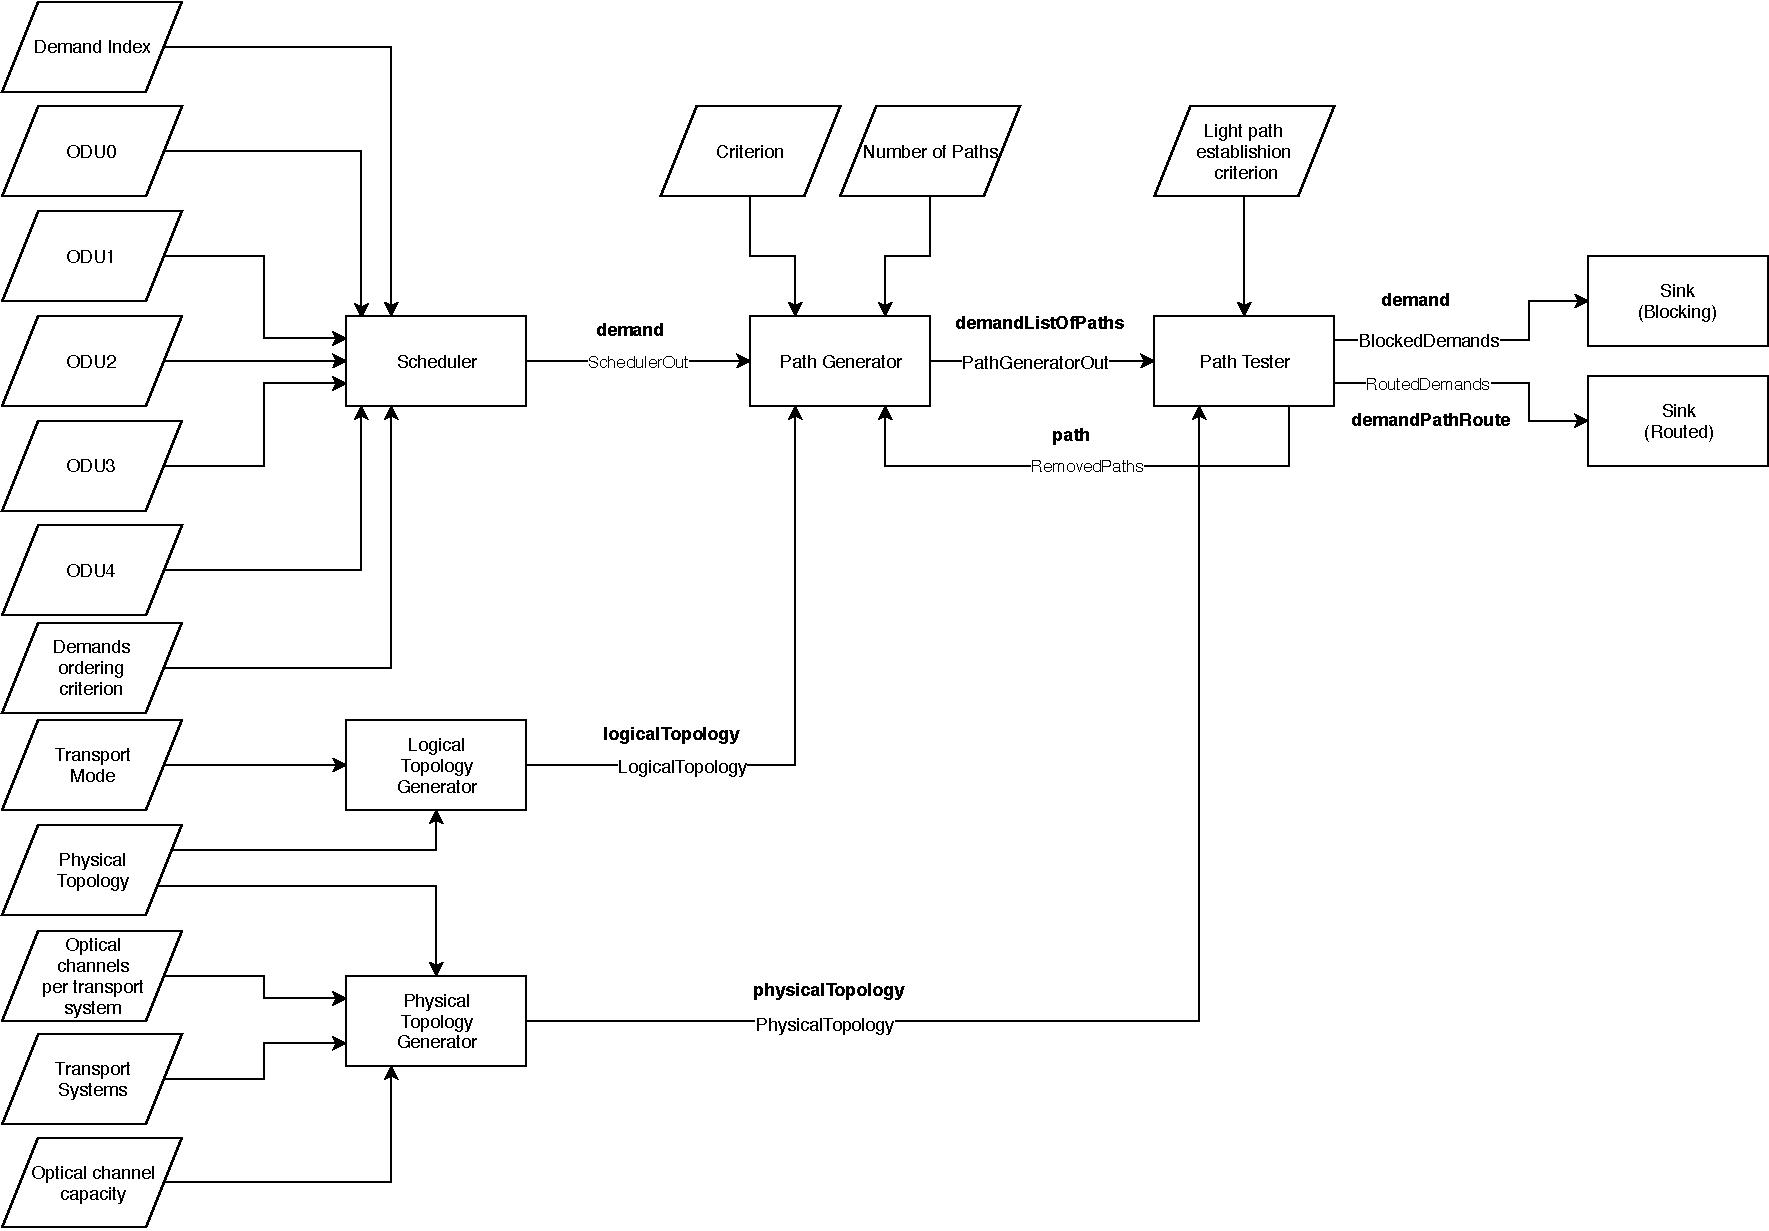
\includegraphics[width=15cm]{sdf/heuristic/transparent/figures/fluxogramaSemGroomingHighLevel}
	\caption{High level diagram of the heuristic algorithm performed.}
	\label{fluxogram_transparent_surv}
\end{figure}

As it is shown in figure 1.112, it is needed a Scheduler block which will be responsible for the creation of an ordered queue containing all the demands entering this network, in an order previously defined (based on the demands ODU type), and ready to be routed.
In order to route those demands there will also be the necessity of a Path Generator block which as its own name implies will create a list of logical paths for each demand between its source and destination nodes, through information received by the Logical Topology Generator block. Next in the Path Tester block where the list of paths previously associated to a demand are tested in order to check their availability in terms of physical capacity in each of the necessary links that comprise the light path used. A Logical and Physical Topology Generators are also needed, the first in order to create the matrix of possible logical connections between nodes and the other to inform us about this network links capacity which will after be continuously updated in the Path Tester block. Finally there are two remaining Sink blocks one to store demands that were routed and their correspondent information and the other to register blocked demands. Both are very usefull to store the information that will later on be present in the final cost report.


%\begin{figure}[H]
%	\centering
%	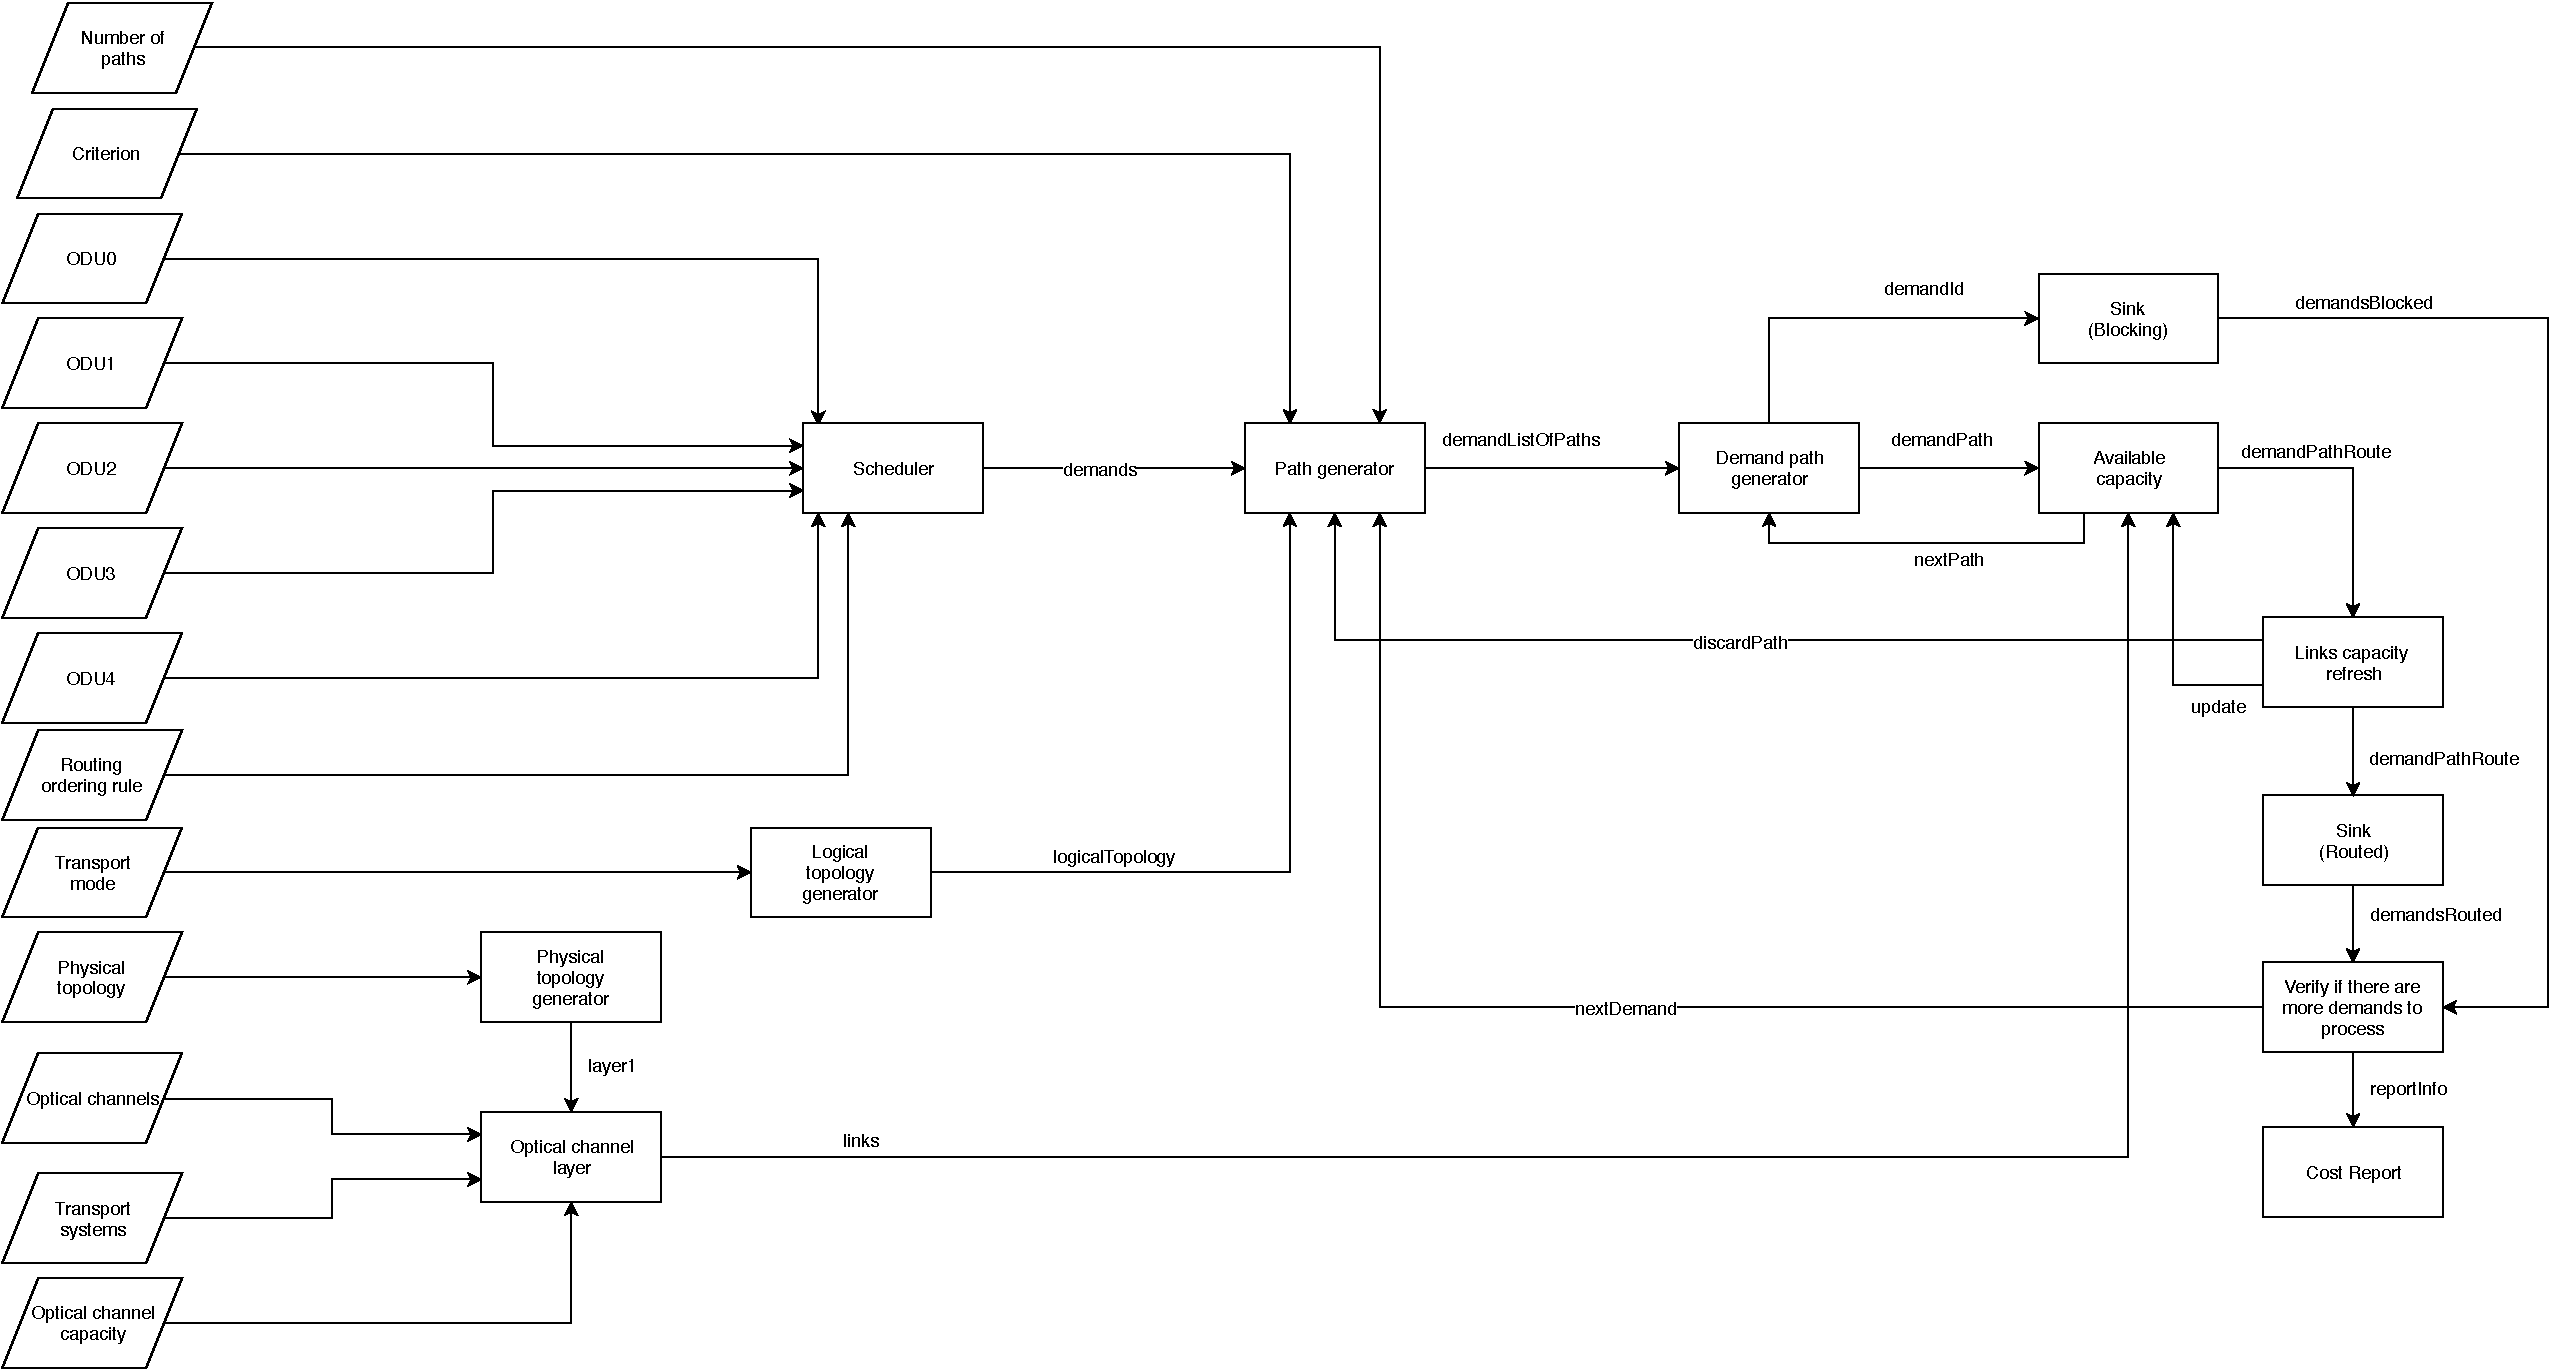
\includegraphics[width=16cm]{sdf/heuristic/transparent/figures/fluxogramaSemGrooming}
%	\caption{Low level diagram of the algorithms performed.}
%	\label{fluxogram_transparent_surv}
%\end{figure}

%Here the main difference is the decomposition of the two super blocks 'Path tester' which is divided in three sub blocks ('Demand path generator', 'Available capacity' and 'Link capacity refresh') and the 'Physical Topology generator' block, divided in two other blocks, all of this in order to better understand their exact functions.

\begin{table}[H]
	\centering
	\begin{tabular}{| c | c | c |}
		\hline
		Signal name & Signal type \\ % it is missing the description of the signals
		\hline
		SchedulerOut &  demand\\ \hline
		LogicalTopology &  logicalTopology\\ \hline
		%layer1 & \\ \hline
		PhysicalTopology & physicalTopology\\ \hline
		PathGeneratorOut &  demandListOfPaths\\ \hline
		RemovedPaths &   path\\ \hline
		BlockedDemands &   demand\\ \hline
		%demandPath & ??? \\ \hline
		RoutedDemands & demandPathRoute\\ \hline
		%demandsRouted & ??? \\ \hline
		%demandsBlocked & ??? \\ \hline
		%update & ??? \\ \hline
		%nextDemand & ??? \\ \hline
		%nextPath & ??? \\ \hline
		%reportInfo & ??? \\ \hline
	\end{tabular}
	\caption{System Signals.}
	\label{system_signals}
\end{table}
	Table 1.20 presents the system signals as well as their type.\\ \\
 \textbf{Signal Types}
\\
\\
\underline{demand}
\\
\begin{table}[H]
	\begin{tabular}{|c|c|c|c|l|}
		\hline
		Demand Index & Source Node & Destination Node & ODU Type & \multicolumn{1}{c|}{Restoration Method}                                                 \\ \hline
		1...$\infty$       & 1...N       & 1...N            & 0...4    & \begin{tabular}[c]{@{}l@{}}0 - None\\ 1 - Protection 1+1\\ 2 - Restoration\end{tabular} \\ \hline
	\end{tabular}
	\caption{Constitution of a demand.}
	\label{demand_variable}
\end{table}
N represents the number of nodes present in the network.\\ \\
\underline{logicalTopology}\\
\\
This is the output signal of the Logical topology generator block, it has a matrix NxN where every logical connection existent between nodes in the network is displayed. In this particular case we are studying the transparent trasnport node so our logical toplogy will be the one presented in table 1.23. In addition here will occur the creation structures corresponding to our network logical links and light paths.\\

\begin{table}[H]
	\centering	
	\begin{tabular}{|c|c|c|c|c|c|c|}
		\hline
		\multicolumn{1}{|l|}{Nodes} & 1   & 2   & 3   & 4   & 5   & 6   \\ \hline
		1                           & \textbf{0}   & 0/1 & 0/1 & 0/1 & 0/1 & 0/1 \\ \hline
		2                           & 0/1 & \textbf{0}   & 0/1 & 0/1 & 0/1 & 0/1 \\ \hline
		3                           & 0/1 & 0/1 & \textbf{0}   & 0/1 & 0/1 & 0/1 \\ \hline
		4                           & 0/1 & 0/1 & 0/1 & \textbf{0}   & 0/1 & 0/1 \\ \hline
		5                           & 0/1 & 0/1 & 0/1 & 0/1 & \textbf{0}   & 0/1 \\ \hline
		6                           & 0/1 & 0/1 & 0/1 & 0/1 & 0/1 & \textbf{0}   \\ \hline
	\end{tabular}
	\caption{Logical Topology Matrix.}
	\label{logical_topology}
\end{table}
\begin{table}[H]
	\centering	
	\begin{tabular}{|c|c|c|c|c|c|c|}
		\hline
		\multicolumn{1}{|l|}{Nodes} & 1   & 2   & 3   & 4   & 5   & 6  \\ \hline
		1                           & \textbf{0}   & 1 & 1 & 1 & 1 & 1 \\ \hline
		2                           & 1 & \textbf{0}   & 1 & 1 & 1 & 1 \\ \hline
		3                           & 1 & 1 & \textbf{0}   & 1 & 1 & 1 \\ \hline
		4                           & 1 & 1 & 1 & \textbf{0}   & 1 & 1 \\ \hline
		5                           & 1 & 1 & 1 & 1 & \textbf{0}   & 1 \\ \hline
		6                           & 1 & 1 & 1 & 1 & 1 & \textbf{0}   \\ \hline
	\end{tabular}
	\caption{Transparent Topology Matrix.}
	\label{Transparentlogical_topology}
\end{table}

\begin{table}[H]
	\centering
	\begin{tabular}{|c|c|c|c|}
		\hline
		Index & Link Source Node & Link Destination Node & Number of Light Paths \\ \hline
		1     & 1...N            & 1...N                 & -1                 \\ \hline
		...   & ...              & ...                   & ...                   \\ \hline
		LO    & 1...N            & 1...N                 & -1                 \\ \hline
	\end{tabular}
	\caption{Logical link variable.}
	\label{logicalLink_variable}
\end{table}

LO represents the number of logical links present in the network.\\ \\
\begin{table}[H]
	\centering
	\begin{tabular}{|c|c|c|c|c|}
		\hline
		Link Index & Light Path Number & Physical Links  & Wavelenght & Capacity (ODU0s) \\ \hline
		1          & 1                 & {[}0/1...0/1{]} & 1...OC     &                  \\ \hline
		...        & ...               & ...             & ...        &                  \\ \hline
		LO         & LP                & {[}0/1...0/1{]} & 1...OC     &                  \\ \hline
	\end{tabular}
	\caption{Light path variable.}
	\label{lightpath_example}
\end{table}
LP represents the number of light paths established in the network.\\
OC represents the number optical channels existent in each physical link.\\
The Physical Links variable inside of the light paths represents the links existent in our network, in this case they can assume two different values, 0 or 1, depending on whether they are used or not to route a demand through a certain light path.\\ \\
\underline{physicalTopology}\\
\\
Here the information about every physical connection existent between nodes and their capacity initially existent is sent to the Path tester block where later on will be updated.

\begin{table}[H]
		\centering
	\begin{tabular}{|c|c|c|c|}
		\hline
		Index & Link Source Node & Link Destination Node & Number of Optical Channels \\ \hline
		1     & 1...N            & 1...N                 & OC                        \\ \hline
		...   & ...              & ...                   & ...                        \\ \hline
		L     & 1...N            & 1...N                 & OC                        \\ \hline
	\end{tabular}
	\caption{Link variable.}
	\label{link_example}
\end{table}

\begin{table}[H]
	\centering
	\begin{tabular}{|c|c|c|c|c|c|}
		\hline
		Link Index & \begin{tabular}[c]{@{}c@{}}Optical Channel\\  Number\end{tabular} & \begin{tabular}[c]{@{}c@{}}Capacity \\ (ODU0s)\end{tabular} & Wavelenght & \begin{tabular}[c]{@{}c@{}}Source\\  Node\end{tabular} & \begin{tabular}[c]{@{}c@{}}Destination\\  Node\end{tabular} \\ \hline
		1...L      & 1...OC                                                           &                                                           & 1...OC    & 1...N                                                  & 1...N                                                       \\ \hline
	\end{tabular}
	\caption{Optical channel variable.}
	\label{opticalChannel_example}
\end{table}


\underline{path}\\

\begin{table}[H]
	\centering
	\begin{tabular}{|c|c|c|c|c|}
		\hline
		Path Index & Source Node & Destination Node & Logical links & Hops\\ \hline
		& 1...N       & 1...N  & [0/1...0/1]  &    \\ \hline
	\end{tabular}
	\caption{Path type signal.}
	\label{path_signal}
\end{table}
The Logical links variable represents the logical links existent in our network, in this case they can assume two different values, 0 or 1, depending on whether they are used or not to route a demand through a certain path.\\ \\
\underline{demandListOfPaths}\\
\\
Inside of the Path Generator block a list of logical paths associated to a pair of source and destination nodes will be created. This paths will depend directly on the logical topology of the network and on the availability of the links.


\begin{table}[H]
		\centering
	\begin{tabular}{|c|c|l|l|}
		\hline
		Demand index           & \multicolumn{3}{c|}{Path index} \\ \hline
		\multirow{3}{*}{1...$\infty$} & \multicolumn{3}{c|}{x}          \\ \cline{2-4}
		& \multicolumn{3}{c|}{x+1}        \\ \cline{2-4}
		& \multicolumn{3}{c|}{x+2}        \\ \hline
	\end{tabular}
	\caption{demandListOfPaths signal.}
	\label{demandListOfPaths_example}
\end{table}

\underline{demandPathRoute}\\
\begin{table}[H]
	\centering
	\begin{tabular}{|c|c|c|c|}
		\hline
		Demand Index           & Path Index             & Physical Link Index                       & 1...L                   \\ \hline
		\multirow{2}{*}{1...N} & \multirow{2}{*}{1...N} & \multirow{2}{*}{Optical Channel} & \multirow{2}{*}{1...OC} \\
		&                        &                                  &                          \\ \hline
	\end{tabular}
	\caption{demandPathRoute signal.}
	\label{demandPathRoute_signal}
\end{table}
%\underline{demandsBlocked}\\
%\begin{table}[H]
%	\centering
%	\begin{tabular}{|c|c|}
%		\hline
%		Demand Index & 1...N \\ \hline
%	\end{tabular}
%	\caption{demandsBlocked signal.}
%	\label{demandsBlocked_signal}
%\end{table}




%\underline{demandPath}\\
%\begin{table}[H]
%	\centering
%	\begin{tabular}{|c|c|l|l|}
%		\hline
%		Demand Index & \multicolumn{3}{c|}{1...N} \\ \hline
%		Path Index   & \multicolumn{3}{c|}{1...N} \\ \hline
%	\end{tabular}
%	\caption{demandPath signal.}
%	\label{demandPath_example}
%\end{table}
Knowing the list of possible shortest logical paths associated to a demand (Dijkstra algotithm), the capacity of the physical links that constitute those logical connections have to be tested. That will occur in the next block of the diagram, the Path Tester block.\\ \\
If there is already an entry in the light path table and if the remaining capacity of that light path, already established, is sufficient to route the demand then our demand is added to that same light path and a demandPathRoute signal is created with information regarding to the demand/path index, route and wavelength used by that same demand. If on the other side the logical path being tested has not enough capacity to process a certain demand or if there is no light path established between that pair of source and destination nodes than an attempt to create another light path entry will be made. If it occurs successfully than a new light path is established in our network and the demand is routed through that same but if there is no possibility of creating a new light path between those nodes than our logical path will have to be ignored and cutted of, and so a next shortest logical path must be tested in the same manner. In order to in further iterations that full path not be considered a path type signal (RemovedPaths) should be created to inform the Path Generator block that those paths must not be considered, this will make the algorithm more efficient. If finally we can not route our demand though none of the logical paths selected then a blocking state occurs, the demand is not routed and a demandsBlocked signal is created. Then finally a cost report is created to obtain a detailed estimation of the network Capex based on user defined equipment costs present on table 1.28.\\ \\

\begin{table}[H]
	\centering
	\begin{tabular}{|c|c|}
		\hline
		Equipment         & Costs      \\ \hline
		OLT               & 15000\euro     \\ \hline
		Transponder       & 5000\euro/GB   \\ \hline
		Optical Amplifier & 4000\euro      \\ \hline
		EXC               & 10000\euro     \\ \hline
		OXC               & 20000\euro     \\ \hline
		EXC Port          & 1000\euro/GB/s \\ \hline
		OXC Port          & 2500\euro/port \\ \hline
	\end{tabular}
	\caption{Equipment costs.}
	\label{equipment_costs}
\end{table}


\begin{table}[H]
	\centering
	\begin{tabular}{|c|c|c|}
		\hline
		\textbf{Parameter} & \textbf{Default value} & \textbf{Description}                                                                                           \\ \hline
		Number of Paths                                                              & 3             & \begin{tabular}[c]{@{}c@{}}Number of paths created between\\ a pair of nodes.\end{tabular}           \\  \hline
		Number of Nodes                                                              & 0             & \begin{tabular}[c]{@{}c@{}}Number of nodes  present\\ in this network.\end{tabular}           \\  \hline
		Routing Ordering Rule                                                        & 0   & \begin{tabular}[c]{@{}l@{}}0 - Descending order\\ 1 - Ascending order\end{tabular} \\ \hline                    
		ODU0                                                                         & Null          & ODU0 demands.                                                                                        \\ \hline
		ODU1                                                                         & Null          & ODU1 demands.                                                                                        \\ \hline
		ODU2                                                                         & Null          & ODU2 demands.                                                                                        \\ \hline
		ODU3                                                                         & Null          & ODU3 demands.                                                                                        \\ \hline
		ODU4                                                                         & Null          & ODU4 demands.                                                                                        \\ \hline
		Criterion                                                                    & Hops          & Shortest path type.                                                                                  \\ \hline
		Transport Mode                                                               & Null          & \begin{tabular}[c]{@{}c@{}}Opaque, transparent or translucid\\ modes.\end{tabular}                   \\ \hline
		Physical Topology                                                            & Null          & \begin{tabular}[c]{@{}c@{}}Physical connections of the\\ network.\end{tabular}                       \\ \hline
		Transport Systems                                                            & 1             & \begin{tabular}[c]{@{}c@{}}Number of transport systems\\ connecting each pair of nodes.\end{tabular} \\ \hline
		Optical Channels                                                             & 100           & \begin{tabular}[c]{@{}c@{}}Optical channels per transport \\ system.\end{tabular}                    \\ \hline
		\begin{tabular}[c]{@{}c@{}}Optical Channel\\ Capacity\end{tabular}           & 100 Gbps      & \begin{tabular}[c]{@{}c@{}}Physical capacity of each \\ channel.\end{tabular}                        \\ \hline
		\begin{tabular}[c]{@{}c@{}}Light Path \\ Establishion Criterion\end{tabular} & to define     & to define                                                                                            \\ \hline
	\end{tabular}
	\caption{System input parameters.}
	\label{system_input}
\end{table}

\begin{table}[H]
	\centering
	\begin{tabular}{|c|c|c|}
		\hline
		\textbf{Block}                                                               & \textbf{Input Parameters}                                                                                                         & \textbf{Input Signals}                                                                \\ \hline
		Scheduler                                                             & \begin{tabular}[c]{@{}c@{}}ODU0, ODU1,ODU2, ODU3, ODU4,\\ Routing Odering Rule, Number of Nodes\end{tabular}                 & None                                                                         \\ \hline
		\begin{tabular}[c]{@{}c@{}}Logical Topology\\ Generator\end{tabular}  & \begin{tabular}[c]{@{}c@{}}Transport Mode, Physical\\ Topology\end{tabular}                                                & None                                                                         \\ \hline
		\begin{tabular}[c]{@{}c@{}}Physical Topology\\ Generator\end{tabular} & \begin{tabular}[c]{@{}c@{}}Physical Topology, Optical Channels,\\ Transport Systems, Optical Channel Capacity\end{tabular} & None                                                                         \\ \hline
		Path Generator                                                        & Number of Paths, Criterion                                                                                                 & \begin{tabular}[c]{@{}c@{}}LogicalTopology,\\ RemovedPaths\end{tabular}      \\ \hline
		Path Tester                                                           & Ligh Path Establishion Criterion                                                                                           & \begin{tabular}[c]{@{}c@{}}PathGeneratorOut,\\ PhysicalTopology\end{tabular} \\ \hline
		Sink (Blocking)                                                       & None                                                                                                                       & BlockedDemands                                                               \\ \hline
		Sink (Routed)                                                         & None                                                                                                                       & RoutedDemands                                                                \\ \hline
	\end{tabular}
	\caption{Blocks input parameters and signals.}
	\label{blocks_input}
\end{table}

\begin{table}[H]
	\centering
	\begin{tabular}{|c|c|c|}
	\hline
	\textbf{Block }                                                                & \textbf{State Variables}                                                                             & \textbf{Output Signals}                                                          \\ \hline
	Scheduler                                                             & \begin{tabular}[c]{@{}c@{}}ODU0, ODU1, ODU2, ODU3,\\ ODU4, Demand Index, \\Number of Demands\end{tabular}        & SchedulerOut                                                            \\ \hline
	\begin{tabular}[c]{@{}c@{}}Logical Topology\\ Generator\end{tabular}  & Logical Topology Matrix                                                                     & LogicalTopology                                                         \\ \hline
	\begin{tabular}[c]{@{}c@{}}Physical Topology\\ Generator\end{tabular} & Physical Topology Matrix                                                                    & PhysicalTopology                                                        \\ \hline
	Path Generator                                                        & \begin{tabular}[c]{@{}c@{}}Logical Topology Matrix,\\ Logical Link, Light Path\end{tabular} & PathGeneratorOut                                                        \\ \hline
	Path Tester                                                           & \begin{tabular}[c]{@{}c@{}}Physical Topology Matrix,\\ Link, Optical Channel\end{tabular}   & \begin{tabular}[c]{@{}c@{}}RoutedDemands,\\ BlockedDemands\end{tabular} \\ \hline
	Sink (Blocking)                                                       & None                                                                                        & None                                                                    \\ \hline
	Sink (Routed)                                                         & None                                                                                        & None                                                                    \\ \hline
\end{tabular}
	\caption{Blocks state variables and output signals.}
	\label{blocks_input}
\end{table}
\clearpage
\textbf{Example:}  \\
\\
Having just 4 optical channels per transmission system, each with a capacity of 100 Gbps, and the following traffic model.

These traffic matrices are represented by ODU0, ODU1, ODU2, ODU3 and ODU4 where each one has a certain bit rate.
The ODU0 corresponds to 1.25 Gbits/s, the ODU1 corresponds to 2.5 Gbits/s, the ODU2 corresponds to 10 Gbits/s, the ODU3 corresponds to 40 Gbits/s and finally the ODU4 corresponds to 100 Gbits/s.
As we can see below, these arrays are bi-directional because they are symmetric arrays and as such, the traffic sent in a certain direction must be the same traffic sent in that opposite direction.

\[
ODU0=
\begin{bmatrix}
0 & 0 & 0 & 0 & 0 & 0 \\
0 & 0 & 0 & 0 & 0 & 0 \\
0 & 0 & 0 & 0 & 0 & 0 \\
0 & 0 & 0 & 0 & 0 & 0 \\
0 & 0 & 0 & 0 & 0 & 0 \\
0 & 0 & 0 & 0 & 0 & 0
\end{bmatrix}
\qquad ODU1=
\begin{bmatrix}
0 & 0 & 0 & 0 & 0 & 0 \\
0 & 0 & 0 & 0 & 0 & 0 \\
0 & 0 & 0 & 0 & 0 & 0 \\
0 & 0 & 0 & 0 & 0 & 0 \\
0 & 0 & 0 & 0 & 0 & 0 \\
0 & 0 & 0 & 0 & 0 & 0
\end{bmatrix}
\]
\[
ODU2=
\begin{bmatrix}
0 & 0 & 0 & 0 & 0 & 0 \\
0 & 0 & 0 & 0 & 0 & 0 \\
0 & 0 & 0 & 0 & 0 & 0 \\
0 & 0 & 0 & 0 & 0 & 0 \\
0 & 0 & 0 & 0 & 0 & 0 \\
0 & 0 & 0 & 0 & 0 & 0
\end{bmatrix}
\qquad ODU3=
\begin{bmatrix}
0 & 0 & 0 & 0 & 0 & 0 \\
0 & 0 & 0 & 0 & 0 & 0 \\
0 & 0 & 0 & 0 & 0 & 0 \\
0 & 0 & 0 & 0 & 0 & 0 \\
0 & 0 & 0 & 0 & 0 & 0 \\
0 & 0 & 0 & 0 & 0 & 0
\end{bmatrix}
\]
\[
ODU4=
\begin{bmatrix}
0 & 0 & 0 & 0 & 0 & 0 \\
0 & 0 & 0 & 9 & 0 & 0 \\
0 & 0 & 0 & 0 & 0 & 0 \\
0 & 9 & 0 & 0 & 0 & 0 \\
0 & 0 & 0 & 0 & 0 & 0 \\
0 & 0 & 0 & 0 & 0 & 0
\end{bmatrix}
\]

\vspace{17pt}
Through these ODU's we can calculate the total network traffic for this specific scenario:\\

$T_1^0$ = 0x1.25 = 0 Gbits/s \qquad
$T_1^1$ = 0x2.5 = 0 Gbits/s \qquad
$T_1^2$ = 0x10 = 0 Gbits/s \\

$T_1^3$ = 0x40 = 0 Gbits/s \quad
$T_1^4$ = 18x100 = 1800 Gbits/s \\

$T_{1}$ = 0 + 0 + 0 + 0 + 1800 = 1800 Gbits/s \qquad
$T$ = 1800/2 = \textbf{900 Gbits/s}\\

Where the variable $T_1^x$ represents the unidirectional traffic of the ODUx, for example, $T_1^0$ represents the unidirectional traffic of the ODU0 and $T_1^1$ represents the unidirectional traffic of the ODU1. The variable $T_{1}$ represents the total of unidirectional traffic that is injected into the network and finally the variable $T$ represents the total of bidirectional traffic.\\

The demands are first ordered in the Scheduler block considering the entry variable, Routing ordering rule (type of ODU), in a single queue. These demands will constitute the SchedulerOut signal.

\begin{table}[H]
	\centering
	\begin{tabular}{| c | c | c | c | c |}
		
		\hline
		 Demand Index  & Source Node & Destination Node & ODU Type & Restoration Method \\
		\hline
		
		1 & 2 & 4 & 4 & 0\\ \hline
		2 & 2 & 4 & 4 & 0\\ \hline
		3 & 2 & 4 & 4 & 0\\ \hline
		4 & 2 & 4 & 4 & 0\\ \hline
		5 & 2 & 4 & 4 & 0\\ \hline
		6 & 2 & 4 & 4 & 0\\ \hline
		7 & 2 & 4 & 4 & 0\\ \hline
		8 & 2 & 4 & 4 & 0\\ \hline
		9 & 2 & 4 & 4 & 0\\ \hline

	\end{tabular}
	\caption{Demands queue generated in the Scheduler block.}
	\label{scheduler_example}
\end{table}

The demands presented in the previous table will be processed from the lowest to highest index.
\\ \\
\textbf{Demand 1}\\ \\

First of all a set of shortest logical paths will be selected based on the logical topology of our network. The paths selected and how many will depend on entry variables, Criterion and Number of Paths, respectively.
Once our shortest logical path is chosen, we must test the same starting by analysing if there is already an entry on our list of light paths established in the network for that logical link or set of links. If there is none or if the existents do not have enough capacity left to transport our demand an effort must be made to create a new entry, that is, create a new lightpath in that logical link or set of links. \\
In this particular case as the list of lightpaths is initially void we must a create a new lightpath using the direct logical link between nodes 2 and 4, if possible.

\begin{figure}[H]
	\centering
	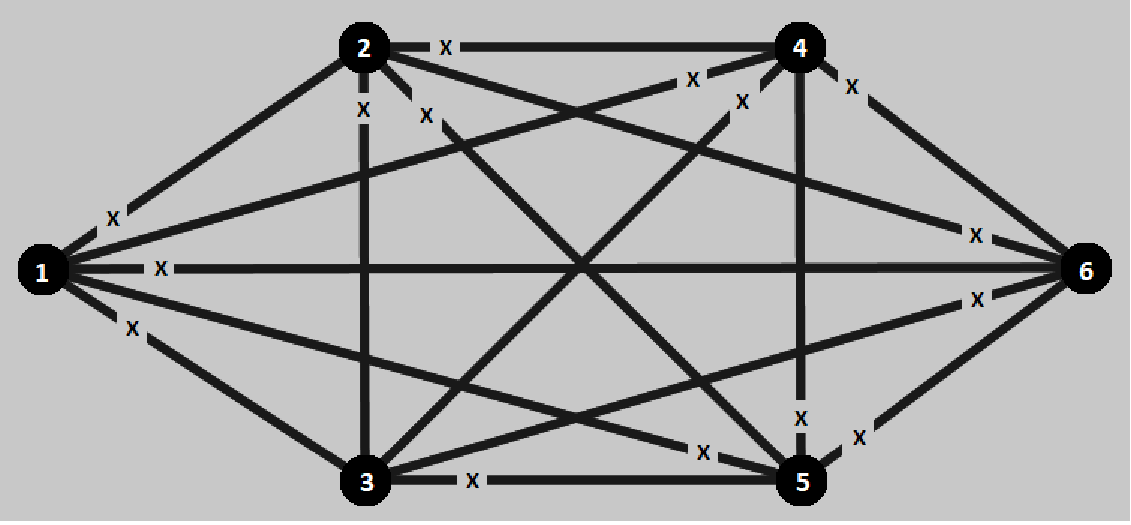
\includegraphics[width=13cm]{sdf/heuristic/transparent/figures/allowed_optical}
	\caption{Allowed optical topology. The allowed optical topology is defined by the transport mode (transparent transport mode in this case). It is assumed that each connections between demands supports up to 4 lightpaths (100 Gbps each).}
	\label{allowed_optical_surv_ref_high_heuristic_transparent}
\end{figure}

\begin{table}[H]
	\centering
	\begin{tabular}{|c|c|l|l|}
		\hline
		Demand index           & \multicolumn{3}{c|}{Path index} \\ \hline
		\multirow{3}{*}{1} & \multicolumn{3}{c|}{1}          \\ \cline{2-4}
		& \multicolumn{3}{c|}{2}        \\ \cline{2-4}
		& \multicolumn{3}{c|}{3}        \\ \hline
	\end{tabular}
	\caption{demandListOfPaths signal.}
	\label{demandListOfPaths_example}
\end{table}

Lets now analyze path number 1, supposedly the shortest one.\\

\begin{table}[H]
	\centering
	\begin{tabular}{|c|c|c|c|c|}
		\hline
		Path Index & Source Node & Destination Node & Logical links & Hops\\ \hline
		1& 2       & 4  & [010000...]  &  1  \\ \hline
	\end{tabular}
	\caption{Path type signal.}
	\label{path_signal}
\end{table}

Since it's constituted only by logical link 2 we must test its capacity in order to analyse the possibility of constituting a new ligth path in logical link number 2.	\\
\\
\underline{Initial values}\\
\begin{table}[H]
	\centering
	\begin{tabular}{|c|c|c|c|}
		\hline
		Index & Link Source Node & Link Destination Node & Number of Light Paths \\ \hline
		2     & 2           & 4                 & 0                \\  \hline
	\end{tabular}
	\caption{Logical link 2.}
	\label{logicalLink_variable}
\end{table}

Since its the first light path to be established in this network the index will be equal to 1. In order to see if there is enough capacity to create this light path we will need to test the physical links that constitutes the very same, in this particular example link number 2.\\

\begin{table}[H]
	\centering
	\begin{tabular}{|c|c|c|c|c|}
		\hline
		Link Index & Light Path Number & Physical Links  & Wavelenght & Capacity (ODU0s) \\ \hline
		2          & 1                 & {[}01000000{]} & 1 & 80    \\ 	\hline
	\end{tabular}
	\caption{Light path 1.}
	\label{lightpath_example}
\end{table}
\begin{table}[H]
		\centering
		\begin{tabular}{|c|c|c|c|}
		\hline
		Index & Link Source Node & Link Destination Node & Number of Optical Channels \\ \hline
		2     & 2            & 4                 & 4                        \\ \hline
		\end{tabular}
	\caption{Physical link 2.}
	\label{link_example}
\end{table}

\begin{table}[H]
\centering
\begin{tabular}{|c|c|c|c|c|c|}
	\hline
	Link Index & \begin{tabular}[c]{@{}c@{}}Optical Channel\\  Number\end{tabular} & \begin{tabular}[c]{@{}c@{}}Capacity \\ (ODU0s)\end{tabular} & Wavelenght & \begin{tabular}[c]{@{}c@{}}Source\\  Node\end{tabular} & \begin{tabular}[c]{@{}c@{}}Destination\\  Node\end{tabular} \\ \hline
	2      & 1                                                           &                              80                             & 1    & 2                                                  & 4                                                       \\ \hline
\end{tabular}
\caption{Optical channel 1 of physical link 2.}
\label{opticalChannel_example}
\end{table}

\underline{Final values}\\ \\
So the final values of these variables after processing demand 1 will be.
\begin{table}[H]
	\centering
	\begin{tabular}{|c|c|c|c|}
		\hline
		Index & Link Source Node & Link Destination Node & Number of Light Paths \\ \hline
		2     & 2           & 4                 & 1                \\  \hline
	\end{tabular}
	\caption{Logical link 2.}
	\label{logicalLink_variable}
\end{table}

\begin{table}[H]
	\centering
	\begin{tabular}{|c|c|c|c|c|}
		\hline
		Link Index & Light Path Number & Physical Links  & Wavelenght & Capacity (ODU0s) \\ \hline
		2          & 1                 & {[}01000000{]} & 1 & 0    \\ 	\hline
	\end{tabular}
	\caption{Light path 1.}
	\label{lightpath_example}
\end{table}

All the available capacity of light path 1 was used so it can not be used to route other demands. Other light paths will have to be created to route demands through this link.

\begin{table}[H]
	\centering
	\begin{tabular}{|c|c|c|c|}
		\hline
		Index & Link Source Node & Link Destination Node & Number of Optical Channels \\ \hline
		2     & 2            & 4                 & 3                        \\ \hline
	\end{tabular}
	\caption{Physical link 2.}
	\label{link_example}
\end{table}

\begin{table}[H]
	\centering
	\begin{tabular}{|c|c|c|c|c|c|}
		\hline
		Link Index & \begin{tabular}[c]{@{}c@{}}Optical Channel\\  Number\end{tabular} & \begin{tabular}[c]{@{}c@{}}Capacity \\ (ODU0s)\end{tabular} & Wavelenght & \begin{tabular}[c]{@{}c@{}}Source\\  Node\end{tabular} & \begin{tabular}[c]{@{}c@{}}Destination\\  Node\end{tabular} \\ \hline
		2      & 1                                                           &                              0                             & 1    & 2                                                  & 4                                                       \\ \hline
	\end{tabular}
	\caption{Optical channel 1 of physical link 2.}
	\label{opticalChannel_example}
\end{table}

